

\documentclass[preprint,12pt]{elsarticle}
\usepackage{caption} 
\usepackage{color}%临时添加,
\usepackage{amssymb,hyperref,booktabs,multirow,multicol,ifthen}
\usepackage{enumerate}
\usepackage{nomencl}
\usepackage{float}
\usepackage{graphics}
\usepackage{framed}


\renewcommand{\nomgroup}[1]
{%Mathematical symbols
\ifthenelse{\equal{#1}{G}}{\item[\textbf{Greek letters}]}{%
\ifthenelse{\equal{#1}{S}}{\item[\textbf{Subscripts}]}{%
\ifthenelse{\equal{#1}{U}}{\item[\textbf{Superscripts}]}{
\ifthenelse{\equal{#1}{C}}{\item[\textbf{Constants}]}{
\ifthenelse{\equal{#1}{M}}{\item[\textbf{Mathematical symbols}]}{
}%几个类别需要几个括号
}
}
}
}%几个类别需要几个括号
}%对应1]
\makenomenclature

 \usepackage{amsmath}%

 \usepackage{lineno}%

\usepackage{bm}%

\captionsetup[figure]{font=small,labelfont=bf,labelsep=period}%

\renewcommand{\figurename}{Fig.}%

\journal{Applied Energy}

\begin{document}

\begin{frontmatter}



\title{A novel 1000\,MW double-reheat ultra supercritical system with turbine-extraction-heated air preheaters and low temperature economizers}


\author[hust,ncst]{Lei Zhang}
\ead{zhanglei@ncst.edu.cn}	
\author[hust]{Jiayi Zhao}
\author[hust]{Tao Yang\corref{cor1}}
\ead{hust\_yt@hust.edu.cn}	
\author[hust]{Yanping Zhang}
\author[hust]{Wei Gao}


\address[hust]{School of Energy and Power Engineering, Huazhong University of Science and Technology, Wuhan 430074,China}
\address[ncst]{College of Metallurgy and Energy, NorthChina University of Science and and Technology, Tangshan 063009,China}
\cortext[cor1]{Corresponding author}

\begin{abstract}%修改到300字以内
Double-reheat ultra-supercritical (USC) unit has received extensive attention for its high efficiency and energy-saving effect.
The optimal design of its thermal system is still under study.
Herein, an optimized system for reasonable fluid heat transfer temperature matching and higher efficiency was proposed.
The novel system used turbine extractions as heat sources of air preheaters and low-pressure economizers to absorb economizer outlet flue gas’ heat, which realized the join optimization of air preheat process and regenerative system.
Models were built to compare energetic performance of the novel system and reference system.
In addition, thermodynamic analyses under partial load operation conditions was conducted. 
Exergy analysis method was used to identify exergy destruction changes of transformed parts and analyze the cause of the change.
Result shows the novel system can largely decrease exergy destruction rate of air preheat process and improve the system's thermal performance.
Furthermore, the novel system increases the temperature of secondary air and reduces the overall superheat degree of several extractions.
Theoretically, the novel system with a overall exergy efficiency of 48.73\%  and reduces the SCE consumption by nearly 5.5\,g/kWh under THA load when the temperature of the flue gas entering the electrostatic precipitator is set to 95$^\circ$C.
Moreover, the novel system can still has advantages in coal saving under partial load condition.
Results indicate that the novel system could improves the performance of double-reheat USC unit and may provide a theoretical basis for its optimization.

\end{abstract}

\begin{keyword}
Double reheat \sep Ultra-supercritical power plant \sep Exergy analysis \sep air preheat process \sep Thermodynamic analyses
\end{keyword}

\end{frontmatter}

\begin{multicols}{2}
\printnomenclature[1.5cm]{}
\end{multicols}



\section{Introduction}
\label{sec1:intro}
Coal is still the main fossil fuel resources for electricity production in the world according to~\cite{Ouedraogo2013Energy}. 
In China, coal–fired power generation accounts for more than 70\% of the total electricity generation and subsequently contribute almost 50\%, 37\%, 33\% and 55\% to the SO$_X$, NO$_X$, dust and CO$_X$ emission volumes respectively~\cite{Zhang2010Analysis}.
Statics show that China has been the largest producer and consumer of energy all over the world since 2013~\cite{Petroleum2014BP}. 
For 2016 as a whole, Chinese coal production fell by 7.9\% and the price of steam coal increased by over 60\%~\cite{Petroleum2017BP}. 
Improve system efficiency and reducing coal consumption is still the main task of power plant design. Nowadays, ultra-supercritical (USC) power plants with large capacity and high parameter are considered to be feasible means to save energy and have rapidly developed word-wide.
The double reheat USC unit is a new generation of USC unit which can improve the thermal performance compared with single reheat units~\cite{Zhao2017Exergy}. 
According to Ref.~\cite{Zhao2017Exergy}, a double reheat unit with the inlet parameter 30.0\,MPa/600/620/620$^\circ$C improves the heat efficiency by 2.4\%-2.6\%, compared with a common used USC unit with the inlet parameter 25.0\,MPa/600/600$^\circ$C.
 The U.S. built the first double reheat unit with main parameter 34.4 MPa/649/566/566$^\circ$C in 1960s.
 Two 700 MW double reheat USC units in Japan were put into operation in 1990. 
 Since 2012, five  double reheat USC units  began to build in China, and three of them put it into operation in 2015.
 Over the past few decades, the double reheat USC units have received more and more attention for its rapid development all over the world.

  

Though the high live steam pressure and temperature of USC unit improves its efficiency, there are still some imperfections which limit the improvement of its performance . 
In order to make an in-depth analysis of the system, Zhao Z et al.~\cite{Zhao2017Exergy} studied the exergy distribution system for a 1000\,MW double reheat USC power plant and provided the main reasons that led to exergy destruction on the steam turbine.
Rashidi et al.~\cite{Rashidi2014Thermodynamic} investigated the thermodynamic analysis of a double reheat steam power plant.
According to Ref.~\cite{Wu2014Component}, component and process based exergy evaluation was performed on a coal-fired power plant in China, which provides guidance for energy-saving strategies.
It pointed out that the exergy destruction in the heat transfer process accounts for the largest proportion.

Compared with common USC system, double-reheat system has some characteristic problems, such as double reheat ratio chose and great superheat degree of the first several extractions.
And some common problems, such as the high boiler exhaust temperature, which leads to unreasonable energy-level matching and great exergy destruction. 

To chose a reasonable reheat parameters, Zhou et al.~\cite{Zhou2016Parametric} carried out parametric analysis and system optimization in double reheat ultra-supercritical power plants based on exergy analysis and economic analysis. The result shows reasonable reheat parameters and reheat stage number can improve  double reheat system's performance.


To reduce the superheat degree of the extractions, Xu et al.~\cite{Xu2015Optimum} investigated the thermal performance of the steam and water cycle with single reheat after the installation of an additional outer steam cooler (AOC).
Results show that the AOC is an effective method to reduce the superheat degree and improve the efficiency of the unit.
Li et al.~\cite{Li2014Thermodynamic} proposed a system adopting 10-stage extractions and two outer steam coolers. 
The result of thermodynamic and techno-economic analyses shows this system can reduce cost of electricity to 55.89 USD/MWh.
Besides, Kjaer~\cite{Kjaer2010A} proposed a regenerative steam turbine to utilize the superheat degree of the extractions.
In this design, part of the extraction from the high pressure turbine enters the additional regenerative steam turbine not the regenerative heater.
Extractions from the intermediate pressure turbine are replaced by those from the regenerative steam turbine.
The superheat degree of the extraction is significantly reduced in this design, and the exergy destruction of regenerative heaters is reduced, which results in an overall improvement in efficiency.

To reuse the energy of the exhaust flue gas, Xu et al.~\cite{Xu2013Techno} proposed a low pressure economizer (LPE) based on the data of some 1000\,MW typical power generation units in China and four possible arrangements of the LPE installation were proposed to compare its energy-saving effects.
Results indicated that LPE connected with higher temperature section of the condensate line brings more reduction of standard coal equivalent (SCE).
Wang et al.~\cite{Wang2012Application} investigated the energy and water saving and the reduction of CO$_2$ after the installation of LPE.
Results show that the optimized measures can bring a reduction of SCE by 2-4\,g/kWh.
Stevanovic et al.~\cite{Stevanovic2014Efficiency} proposed an additional high pressure economizer installed at a long term running lignite-fired power plant.
Results show that more than 30\,MW of the flue gas waste heat is recovered, which brings an improvement in gross efficiency by 0.53\% and 9.4\,MW extra output power.
Xu et al~\cite{Xu2013A} made the air preheater divided into two stages to reduce the temperature difference in heat transfer process.
Besides, a LPE is installed between the two air preheaters to obtain an appropriate flue gas temperature range.
Thermodynamic and Technic-economic analysis are conducted to reveal the performance improvement.
It was found that the SCE consumption can be reduced by 6.7\,g/kWh. 

The installation of LPE have some other benefit such as improve The electrostatic precipitator collection efficiency~\cite{Li2016Low}.

Due to  boiler design and thermal system design belong to deferent research area, boiler has been studied as a whole and ignored the joint optimization of boiler heat transfer process and regenerative process.

In this paper, a novel system based on a 1000\,MW double reheat USC reference system  is proposed to realize boiler and regenerative system energy cascade utilization. 
The novel system realized reasonable temperature matching of flue gas, air, extraction steam and condensate water by using turbine-extraction-heating air preheaters (EAPHs) and LPEs.
Specifically, the main works of this study include: (1)Modeling the novel system and reference system with EBSILON® Professional; (2) Using exergy analysis to compare both systems' exergy efficiency , exergy destruction distribution and subsystems performance change;(3) Analyzing both systems' thermal performance under off-design conditions.



\section{System optimization of double reheat USC system}
\label{sec2:system intro}
\subsection{Reference system on operation} % (fold)
\label{sub2:ref intro}
A typical coal-fired double reheat USC power plant in operation is chosen as the reference unit.
The parameter settings at maximize continuous power are 310\,bar/600$^\circ$C for the main steam, 610$^\circ$C for the reheat steam pressure, 33.5\% for the proportion of the single reheat steam pressure to the main steam pressure, and 33\% for the proportion of the double reheat steam pressure to the single reheat steam pressure~\cite{Zhao2017Exergy}.
The output power of the reference system under the design condition is 1000 MW.
The unit consists of one super high pressure cylinder (VHP), one high pressure cylinder (HP), one intermediate pressure cylinder (IP), and two low pressure cylinders (LPs).
Regenerative system with four high pressure regenerative heaters (HRHs), five low pressure regenerative heaters (LRHs), and one deaerator (DEA) are adopted.
Besides, two additional outer steam coolers (AOC1, AOC2) are used to cool two extractions due to its high super-heating degree. The exhaust steam pressure of the steam turbine is set 4.5\,kPa. The simplified schematic of it is presented in Fig.~\ref{fig:reference_system}.

\begin{figure}[htbp]
\centering
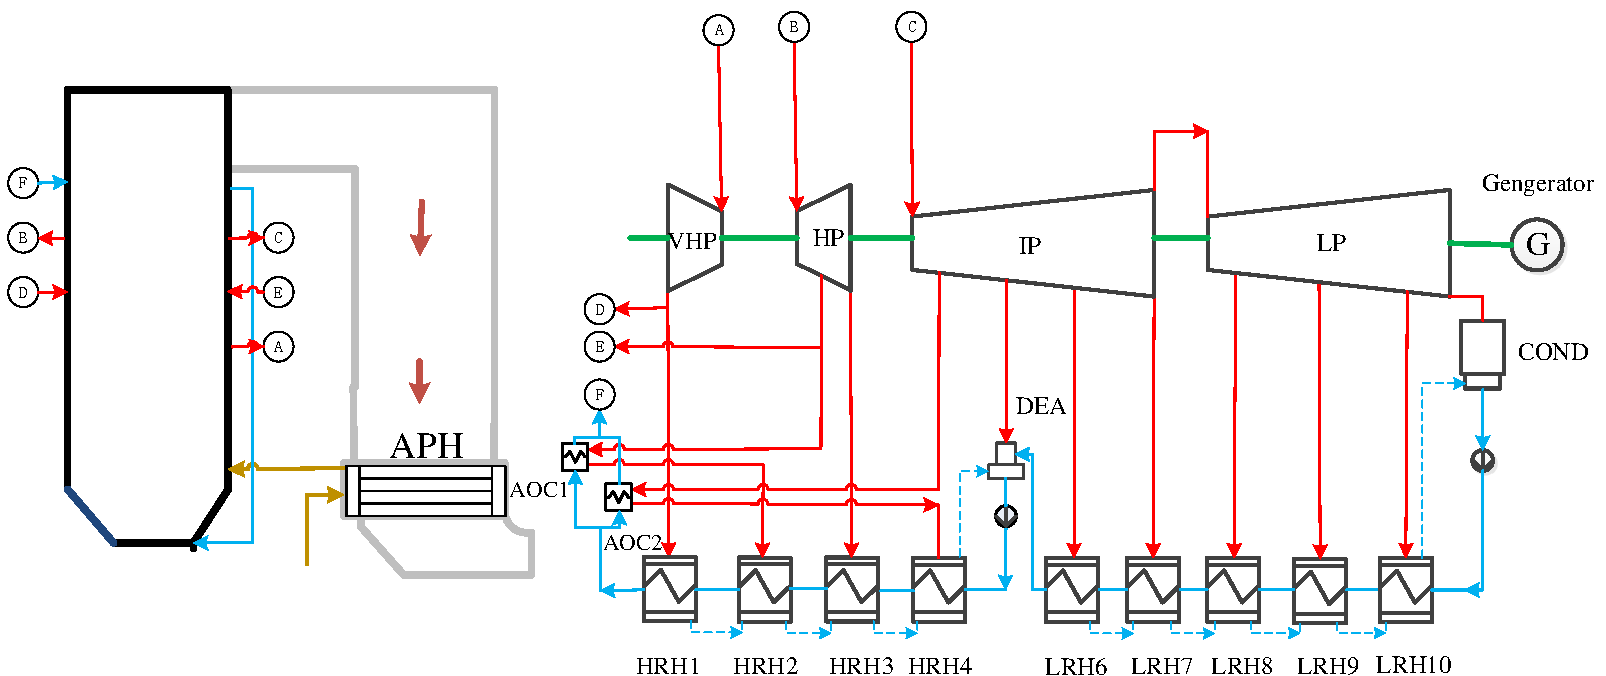
\includegraphics[width=1\textwidth]{fig/reference_system}
\caption{Schematic of the reference system} 
\label{fig:reference_system}
\end{figure}
%从参考系统的锅炉虽然仍然采用Π型布置,但其内部受热面和传统一次再热锅炉有较大区别。
The system's boiler heat transfer surfaces arrangement is shown in Fig.~\ref{fig:boiler_surface}. 
The boiler furnace is composited by the membrane wall, along flue gas flow direction lays low-temperature superheater (Lts) screen tube, cold segment of high-temperature first reheater (Csf), cold segment of high-temperature second reheater (Css), High temperature super-heater (Hts), hot segment of high-temperature first reheater (Hsf), hot segment of high-temperature second reheater (Hss).
After Hsf and Hss the flue gas channel is divided into the front-duct flue and the back-duct flue.
The front duct arranges low-temperature first reheater (Ltfr) and the front-duct economizer (Feco).
The back duct arranges low-temperature second reheater (Ltsr) and the back-duct economizer (Beco).
(air preheater)APH is arranged in vertical shaft.

From the arrangement of heating transfer surfaces, the boiler can be divided into two parts: the part achieving heat absorption of water/steam process in the furnace, and the APH to complete the air preheat process.
It can be seen that most heating surfaces of boiler is arranged in the furnace, while the horizontal flue and vertical shaft are only equipped with APH.
So the horizontal flue and vertical shaft have sufficient space to install other equipments.

\begin{figure}[htbp]
\centering
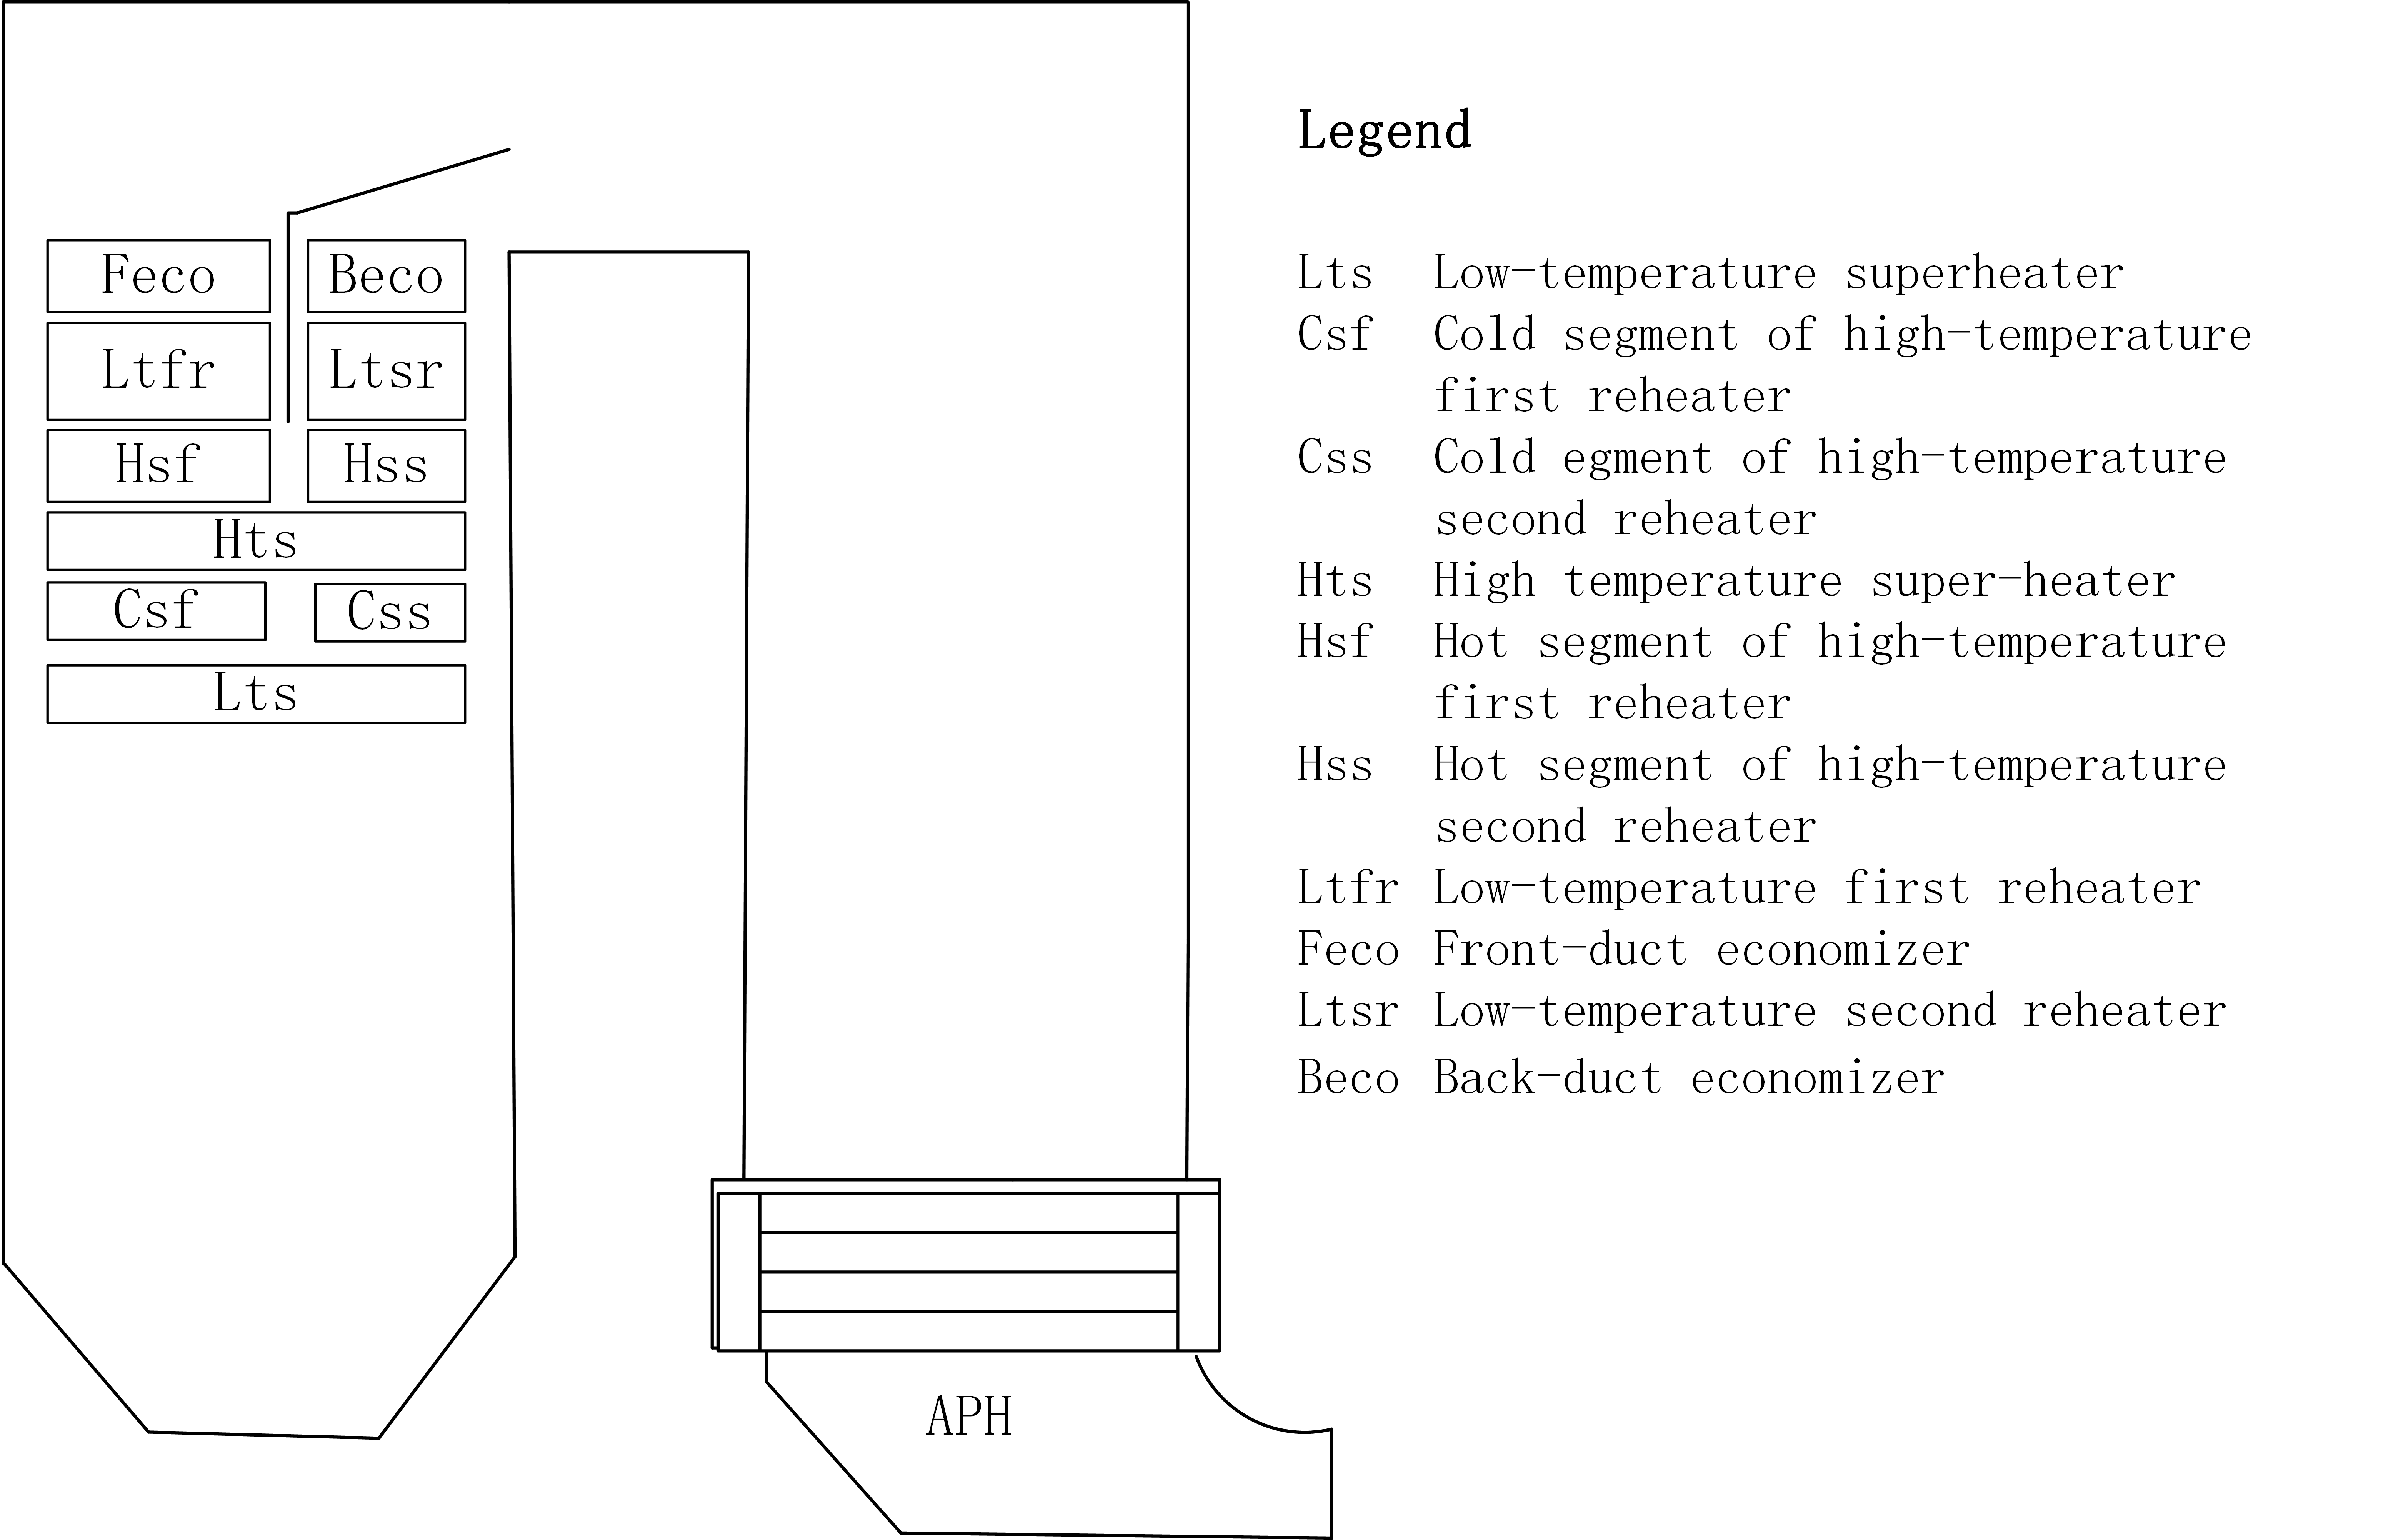
\includegraphics[width=0.9\textwidth]{fig/boiler_surface.png}
\caption{Boiler heat transfer surfaces layout} 
\label{fig:boiler_surface}
\end{figure}


The main parameters of the reference system are shown in Table~\ref{tab:ref input}.

\begin{table}[htbp]
\caption{The main input parameter of reference system }
\label{tab:ref input}
\centering
\begin{tabular}{lll}
\toprule 
Items & Unit & Value\tabularnewline
\midrule
 Live steam mass flow rate 	    	&t/h 			&2533 \\
 Live steam pressure 		    	&bar 			&310\\
 Live steam temperature		     	&$^\circ$C		&600		\\
 First reheat steam pressure    	&bar			&100.9		\\
 First reheat steam temperature  	&$^\circ$C		&610		\\
 Second reheat steam pressure    	&bar			&30.8		\\
 Second reheat steam temperature 	&$^\circ$C		&610		\\
 Power generation output 			&MW				&1000		\\
\bottomrule
\end{tabular}	
\end{table}

Table~\ref{tab:reheater parameter} gives the temperature profiles of regenerative heaters and the air preheater, revealing their energy match level.
For the APH, the temperature of flue gas at the inlet is 376$^\circ$C under, while the temperature of the air to be heated by the flue is 23$^\circ$C.
The logarithm mean temperature difference (LMTD) of the APH is calculated to be 72$^\circ$C.
Compared with the air preheater, the regenerative heaters have much lower LMTD from 6.88$^\circ$C-15.87$^\circ$C.
According to the second law of thermodynamics, the bigger the temperature difference the greater the irreversible loss.
So it needs to optimize the air preheat process to reduce energy loss of the system.
AOC1 and AOC2 face the same problem of high LMTD compared with RHs.
It's better to find a way to make double reheat USC system's high temperature extractions a reasonable arrangement.



\begin{table}[htbp]
\caption{Fluid parameters of regenerative heaters and air preheater}
\label{tab:reheater parameter}
\centering
\begin{tabular}{llll}
\toprule 
\multirow{2}{2cm}{Components} &\multirow{2}{2.7cm}{Hot fluid temperature($^\circ$C)}  & \multirow{2}{3.2cm}{Cold fluid temperature ($^\circ$C)}&\multirow{2}{2.2cm}{LMTD ($^\circ$C)}\tabularnewline
&&&\tabularnewline
\midrule
APH  &  376.00 	& 23.00  & 72.4\tabularnewline
AOC1 &   526.56 & 304.51 & 69.75\tabularnewline
AOC2 &  527.48 	& 304.51 & 60.81\tabularnewline
HRH1 &   417.07 & 273.62 & 10.64\tabularnewline
HRH2 &   314.53 & 240.73 & 10.77\tabularnewline
HRH3 &   434.54 & 205.89 & 12.68\tabularnewline
HRH4 &   316.51 & 186.48 & 6.88\tabularnewline
LRH6 &  394.01 	& 140.46 & 13.19\tabularnewline
LRH7 &   313.17 & 104.49 & 15.87\tabularnewline
LRH8 &   191.84 & 82.42  & 9.82\tabularnewline
LRH9 &   116.61 & 59.25  & 10.03\tabularnewline
\bottomrule
\end{tabular}
\end{table}




\subsection{Proposal of a novel system with EAPHs and LPEs}
\label{sub2:prop novel sys}

To reduce the energy loss caused by APH, a novel system is proposed, in which air is not heated by flue gas in the conventional air preheater, but 8 turbine-extraction-heated air preheaters (EAPH1-EAPH8).
The layout of the optimization system is presented in Fig.~\ref{fig:novel_system}.

As shown in Fig.~\ref{fig:extraction_heat_APH}, the extracted steam divides into two parts, one is sent to the regenerative heater to heat the condensate or feedwater and the other one is sent to corresponding EAPH to heat air.
The drainage from the air preheater joins with that of corresponding regenerative heater after finishing heat transfer .
Steam distribution ratio is determined according to EAPH upper terminal temperature difference settled in the system.
It should be mentioned that not all the extractions are available for air heating.
The last two stage extractions' pressure are much lower than barometric pressure which has a great risk of air leakage into the steam, and APH8 shall be shut down under low load for the same reason.

The AOCs in the reference system are designed to heat feedwater.
Although AOC inlet steam has a great supper heat degree, the small heat exchanged makes feedwater have little temperature rise.
So the LMTD is very high in AOCs.

To reduce rise AOCs' exergy efficiency and the superheat degree of extractions entering the heat exchangers, four additional outer steam coolers (AOC1-AOC4) are installed at the air side outlet of EAPH1.
Air side outlet of EAPH1 will sent to boiler as secondary air, which has small mass quantity and lower heat capacity compared with feedwater. 
So the secondary air temperature can make a remarkable rise, and LMTD of AOCs can get down.
Extractions from the 2nd to the 5th have very high temperature and great superheat degree, they are sent to AOCs in the order of temperature level.
For example, the 2nd extraction has the highest temperature, and is applied to heat the air in the 1st AOC, and then the cooled steam from AOC1 is sent to HRH2 and air EAPH2 to heat the water and air respectively.  

\begin{figure}[htbp]
\centering
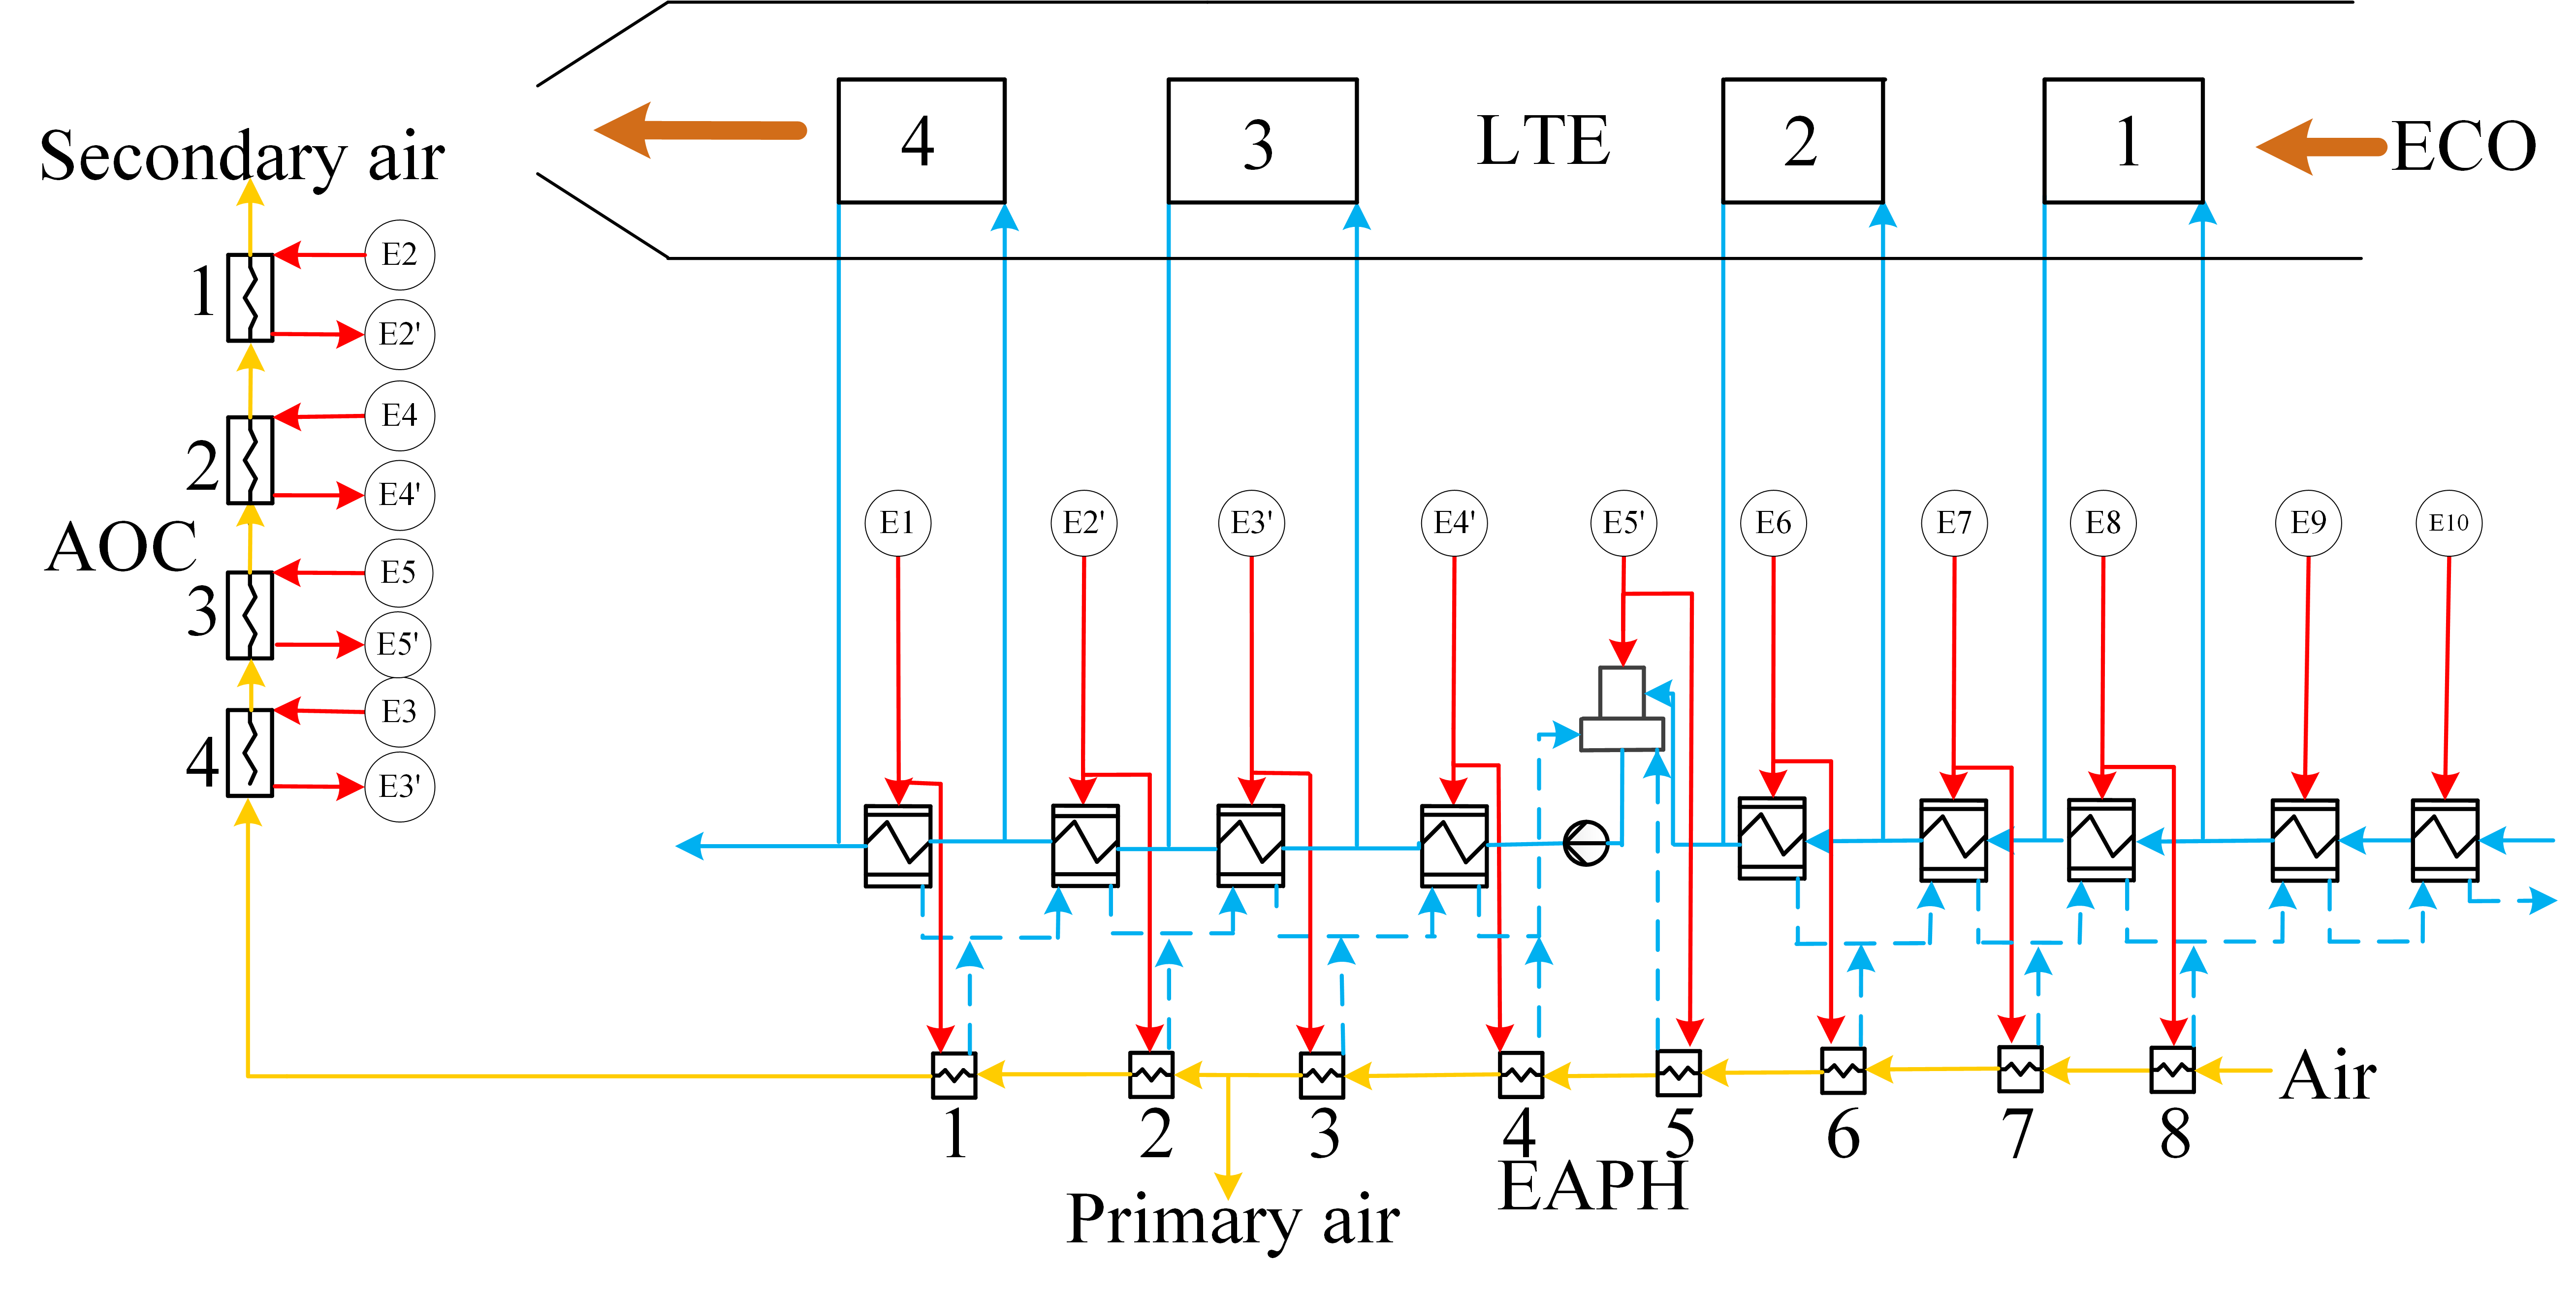
\includegraphics[width=1\textwidth]{fig/novel_system.png}
\caption{Schematic of the novel system} 
\label{fig:novel_system}
\end{figure}

\begin{figure}[htbp]
\centering
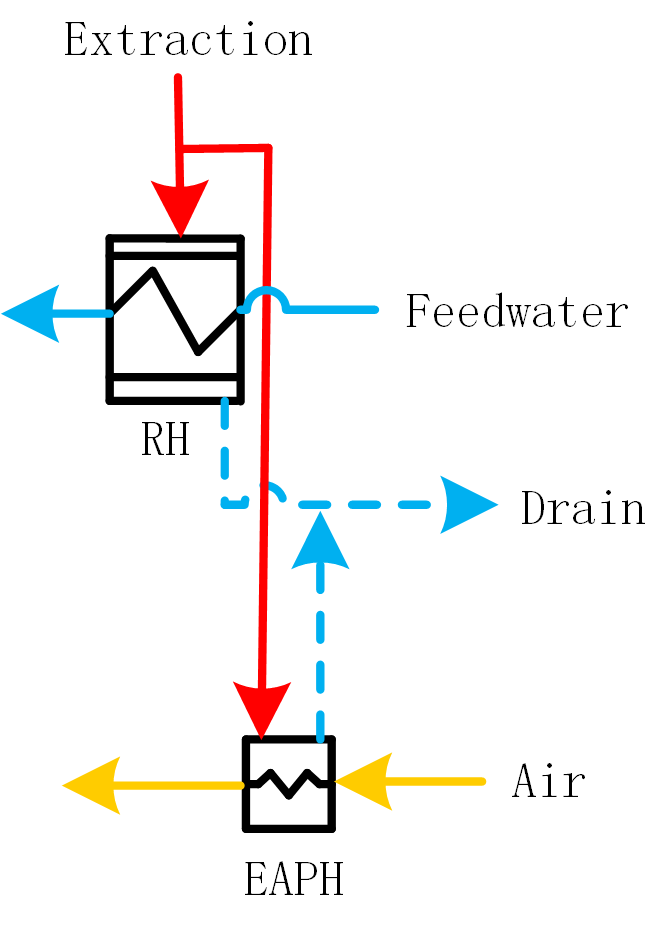
\includegraphics[width=0.3\textwidth]{fig/extracion_heat_APH.png}%extraction_heat_APH
\caption{Process flow diagram of RH and EAPH} 
\label{fig:extraction_heat_APH}
\end{figure}

Cause removing of the APH originally installed in the vertical shaft, the flue gas's heat needs to be absorbed by other means.
As shown in Fig.~\ref{fig:novel_system}, the flue gas at the outlet of economizer is utilized to heat the condensate and feed water by four LPEs, which are paralleled to HRH2, HRH4, LRH6, and LRH8 respectively. 
Part of the condensate and feed water at the inlet of regenerative heater are sent to the LPE, then the heated water join with corresponding regenerative heater's outlet water. 
Considering the acid dew point temperature, the flue gas temperature at the outlet of the last LPE can be set 95$^\circ$C. 


% \section{Model establishment and thermodynamic evaluation} % (fold)
% \label{sec3:modle est and eval}
\section{Model description and Thermodynamic metric}
\label{ssub:model_establishment_and_system_analysis_method}

\subsection{Model establish method and main assumption}
\label{ssub3:modle description}
%对模型中如何基于现有系统进行的改造,和哪些数据不发生变化进行说明
%添加模型中基本部件的特性 添加个表格
In this paper, the thermodynamic cycle of the thermal system under different loads are simulated with EBSILON® Professional.
EBSILON is a power plant simulation tool which can calculate thermodynamic quantities and widely used in power plant system model establishment and analysis~\cite{Li2015Integrated,Yao2017Multi}. 
The simulation model gives the detailed data with high degree of reliability to calculate the thermodynamic state.
While use this software simulating systems, main equipments work flow parameters and some basic properties need to be settled.
Cause designed based on the reference system, the novel system's main input parameters(such as live steam parameters, fist/second reheat steam parameters and turbine extractions parameters) keeps the same as it, which can be find in Table~\ref{tab:ref input} and Table~\ref{table:extractions_parameter}.
Based on the practice, the upper temperature differences of novel systems' LPE, AOC and EAPH are settled to 30$^\circ$C, 20$^\circ$C and 5$^\circ$C. 
And other main components model details are give in Table~\ref{table:model_details}. 

\begin{table}
\caption{Model details of main components}
\label{table:model_details}
\begin{centering}
\begin{tabular}{ll}
\toprule 
Components 				& Model details\tabularnewline
\midrule
Boiler         			& Economizer out let flue gas temperature =376\textcelsius ;\tabularnewline
 						& Slag temperature =850\textcelsius ;\tabularnewline
 						& Combustion efficiency = 0.99.\tabularnewline
Turbine 				& Isentropic efficiencies are from 0.83 to 0.93, \tabularnewline
 						& calculated from thermal equilibrium diagram.\tabularnewline
Condenser 				& Upper terminal temperature difference = 5\textcelsius .\tabularnewline
Regenerative reheats 	& Upper terminal temperature differences are from -1.7\textcelsius{}  \tabularnewline
 						& to 2.2\textcelsius ,calculated from thermal equilibrium diagram.\tabularnewline
\bottomrule
\end{tabular}
\par\end{centering}
\end{table}

On the off-design conditions, EBSIOLON's simulation and parameter calculation of the equipment, such as turbine, is based on experimental characteristics of units.
However, only turbine's off-design characteristic curves can actually be obtained,and boiler's and heat exchangers' data can not be gotten.
It has to be replaced by built-in data.
It’s needed to assume that the difference between the built-in data and the actual data to meet the error requirements.
The following assumptions need to be made in order to be able to simulate correctly.
\begin{enumerate}[(1)]
\item Both novel and reference systems are operated in stable condition.
\item The thermal efficiency of the equipment is calculated from the thermal balance of the input and output parameters of the components, assuming that the calculation error requirement can be met.
\item According to the heat map, set the upper and lower end difference of the heat exchanger as a fixed value, and do not change during different load conditions' simulation.
\item Do not take the pips' complexity and equipment’s installation difficulty of the novel system as consideration.
\end{enumerate}
More detail descriptions of the thermaldynamic model of involved components can be found in Ref.~\cite{Yao2017Multi}.

\begin{table}
\caption{The turbine extractions parameters on design condition}
\label{table:extractions_parameter}
\begin{centering}
\begin{tabular}{cccccc}
\toprule 
\multirow{2}{*}{Extractions} & Pressure & Temperature & \multirow{2}{*}{Extractions} & Pressure & Temperature\tabularnewline
 & (bar) & (℃) &  & (bar) & (℃)\tabularnewline
\midrule
1st & 107.89  & 429.00 & 6th & 7.15  & 394.01 \tabularnewline
2nd & 61.89 & 528.30  & 7th & 3.90  & 313.17\tabularnewline
3rd & 34.34 & 435.20  & 8th & 1.23  & 191.84\tabularnewline
4th & 17.56  & 526.55  & 9th & 0.57  & 116.61\tabularnewline
5th & 10.35  & 447.37 & 10th & 0.21 & 62.57\tabularnewline
\bottomrule
\end{tabular}
\par\end{centering}
\end{table}

\subsection{Thermodynamic metric} %(fold)
\label{ssub3:analsys method} 
%为了能够对优化系统与参考系统进行评估,揭示系统优化的内在机理,本文引入热力学第二定律的分析方法即用分析方法。
Based on the second law of thermodynamics, exergy analysis method is widely used in power plant thermal system analysis and optimization~\cite{Si2017Exergy,Yang2013Comprehensive,Ahmadi2016Energy}
Exergy analysis, is adopted to reveal the location, the magnitude and the sources of thermodynamic inefficiencies of the unit.
Usually, exergy destruction and exergy efficiency are chosen as evaluation indices of the thermal system or an individual component, 
The general exergy balance of component or system can be expressed in the following form:
\begin{equation}
\label{equation:1}
\dot{I}=\sum\dot{Ex}{}_{in}-\sum\dot{Ex}{}_{out}+\sum\dot{W}{}_{in}-\sum\dot{W}{}_{out}
\end{equation}





Exergy efficiency can be calculated in the following form:
\begin{equation}
\label{equation:2}
\eta_{\uppercase\expandafter{\romannumeral2}}=\frac{\dot{Ex}{}_{earned}}{\dot{Ex}{}_{cost}}
\end{equation}
For different equipment under stable operating conditions, equation~\ref{equation:1}, ~\ref{equation:2} have different forms as shown in Table~\ref{tab:exergy equation}~\cite{Aljundi2009Energy}

\begin{table}
\caption{Exergy analysis equations for power plant components}
\label{tab:exergy equation}
\centering
\begin{tabular}{lll}
\toprule 
 & Exergy destruction rate  & Exergy efficiency\tabularnewline
\midrule
Boiler & $\dot{I}_{boiler}=\dot{Ex}{}_{fuel}+\dot{Ex}{}_{in}-\dot{Ex}{}_{out}$ & $\eta_{\uppercase\expandafter{\romannumeral2},boiler}=\frac{\dot{Ex}{}_{out}-\dot{Ex}{}_{in}}{\dot{Ex}{}_{fuel}}$\tabularnewline
Pump & $\dot{I}_{pump}=\dot{Ex}{}_{in}-\dot{Ex}{}_{out}+\dot{W}{}_{pump}$ & $\eta_{\uppercase\expandafter{\romannumeral2},pump}=1-\frac{\dot{I}_{pump}}{\dot{W}{}_{pump}}$\tabularnewline
Heater & $\dot{I}_{heater}=\dot{Ex}{}_{in}-\dot{Ex}{}_{out}$ & $\eta_{\uppercase\expandafter{\romannumeral2},heater}=1-\frac{\dot{I}_{heater}}{\dot{Ex}{}_{in}}$\tabularnewline
Turbine & $\dot{I}_{turbine}=\dot{Ex}{}_{in}-\dot{Ex}{}_{out}-\dot{W}{}_{el}$ & $\eta_{\uppercase\expandafter{\romannumeral2},turbine}=1-\frac{\dot{I}_{turbine}}{\dot{Ex}{}_{in}-\dot{Ex}{}_{out}}$\tabularnewline
Condenser & $\dot{I}_{condenser}=\dot{Ex}{}_{in}-\dot{Ex}{}_{out}+\dot{W}{}_{pump}$ & $\eta_{\uppercase\expandafter{\romannumeral2},boiler}=\frac{\dot{Ex}{}_{out}}{\dot{Ex}{}_{in}+\dot{W}{}_{pump}}$\tabularnewline
Cycle &$\dot{I}_{total}=\dot{Ex}{}_{fuel}-\dot{W}{}_{net,out}$ & $\eta_{\uppercase\expandafter{\romannumeral2},total}=\frac{\dot{W}{}_{net,out}}{\dot{Ex}{}_{fuel}}$\tabularnewline
\bottomrule
\end{tabular}
\end{table}

For flue gas, air, water and steam, the specific exergy can be calculated by equation~\ref{equation:3}.

\begin{equation}{}
\label{equation:3}
ex=h-h_{0}-T_{0}\left(s-s_{0}\right)
\end{equation}
Then the total exergy rate associated with fluid stream becomes:
\begin{equation}
\dot{Ex}=\dot{m}x=\dot{m}\left[h-h_{0}-T_{0}\left(s-s_{0}\right)\right]{}
\end{equation}
The fuel specific exergy calculate method~\cite{Yan2016The} can be expressed as.
\begin{equation}
ex_{fuel}=LHV\left(1.0064+0.1519\frac{H}{C}+0.0616\frac{O}{C}+0.0429\frac{N}{C}\right)
\end{equation}
Where LHV refer to lower heating value of fuel, C, H, O, N refer to mass fraction of carbon, hydrogen, oxygen, nitrogen by element analysis.
More details of power plant equipments' exergy  efficiency calculation can be found in Ref.~\cite{G2016Exergy}

In order to clearly analyze the effect of system optimization, this paper divides the double-reheat USC system into four main subsystems and a sum of all other equipments, valves and pips named "other".
The four main subsystems are: boiler with out APH, turbine, air preheat subsystem and regenerative subsystem.
The equations mentioned above can also be used into exergy analysis of these four main subsystems.
For the "other" part, this paper used counter balance analysis method to calculate its exergy destruction rate, which means subtract the share of the four main subsystems from the total exergy destruction.
The exergy destruction rate can be calculated by using equation as follows:

\begin{equation}
\dot{I}_{other}=\dot{I}{}_{total}-\sum\dot{I}{}_{subsystems}
\end{equation}


\section{Thermodynamic performance evaluation} % (fold)
\label{sub:Thermodynamic_evaluation}
%对word版本的分布进行了较大的改动,需要继续调节
\subsection{Thermodynamic comparison in design condition}
\label{ssub:desing_compare}
%表四
The comparison of thermal dynamic performance between these two systems is given in Table~\ref{table:thermal performance compare}. 
Under design condition, the novel system brings an improvement of net generating power by 11.02 MW, and reduces SCE consumption by 5.5\,g/kWh.
The power generation efficiency reaches 48.73\%, and 1.04\% higher then that of reference system.
Meanwhile, the exergy efficiency of novel system is 1.01\% higher, showing good exergy-saving effect. 

\begin{table}
\caption{Thermodynamic performance of reference and novel systems}
\label{table:thermal performance compare}
\centering
\begin{tabular}{p{7.5cm}p{1.75cm}p{1.75cm}}
\toprule 
Items & Reference system & Novel system\tabularnewline
\midrule
Net generating power (MW) & 999.10 & 1011.19\tabularnewline
Generating efficiency (\%) & 47.69 & 48.73\tabularnewline
Addition in generating efficiency (\%) &  & 1.04\tabularnewline
Standard coal consumption rate (g/kWh) & 257.59 & 252.10\tabularnewline
Reduction in standard coal consumption rate (g/kWh) &  & 5.49\tabularnewline
Exergy efficiency (\%) & 46.51 & 47.52\tabularnewline
Addition in exergy efficiency (\%) &  & 1.01\tabularnewline
\bottomrule
\end{tabular}
\end{table}
% 根据用损失对比表从新进行分析,从为什么锅炉空预器效率提高,其他不变或者降低说起
Table~\ref{table:system exergy campare} gives the results of subsystem exergy analysis of the two system. 
It is found that the novel system has an improvement in exergetic performance by an decrease of 10.82\,MW of total exergy destruction rate.
Exergy destruction rate of boiler accounts for the highest proportion and decrease most (11.04\,MW).
Air preheat subsystem's exergy destruction rate changes from 27.39\,MW to 16.55\,MW, having a 10.84\,MW decrement, having the largest Optimization ratio.
In the mean time, turbine and regenerative subsystem have a relatively small change at about 1\,MW. 

The item "other" of novel system is higher then reference system, showing that the uncalculated components of systems have a increment of exergy destruction rate.
Among the uncalculated components, the pips' amount increasing and  parameters unmatched work fluid mixing are the main reason why that part has a increment in exergy destruction rate.

\begin{table}
\caption{Exergy destruction rate comparison of reference and novel systems }
\label{table:system exergy campare}
\centering
\begin{tabular}{lll}
\toprule 
Items & Reference System\,(MW) & Novel System\,(MW)\tabularnewline
\midrule 
Boiler(without AP) & 883.26 & 872.22\tabularnewline
Turbine & 63.33 & 63.97\tabularnewline
Air preheat subsystem  & 27.39 & 16.55\tabularnewline
Regenerative subsystem & 22.53 & 21.56\tabularnewline
Other & 131.03 & 142.42 \tabularnewline
Total & 1127.54 & 1116.72\tabularnewline
\bottomrule
\end{tabular}
\end{table}

% 下面两段话需要根据图修改

%本文是针对空预系统和回热系统的联合优化改造,所以本文将新系统和参考系统中的差变化,系统中设备的效率和用损变化进行了分析。
To get in-depth analysis of both systems, research of the mainly optimized subsystems: air preheat subsystem and regenerative subsystem was conducted.
Table~\ref{table:extraction_compare} gives the variation of mass flow rate of extractions.
As illustrated in Table~\ref{table:extraction_compare}, mass flow rate of the 1st, 3rd, 5th and 8th extractions of the novel system is more than that of the reference system, and the rest extractions except the last two, has the opposite variation. 
It can be found that the impact of system optimization on extraction is twofold: air is heated by extractions, which will cause an increment in mass flow, and the use of LPE can saves extractions so the total extraction mass flow keeps almost unchanged.

The sum of 4th to 10th extractions mass flow increases from 138.46 kg/s to 145.07 kg/s, and the 8th extraction increase 13.9 kg/s.
The mass flow increase of low pressure extractions implies that novel system can modify the quantity distribution of extractions.

%新系统优化可二次再热后蒸汽的抽汽,使8th抽汽量增加
\begin{table}
\caption{Extractions comparison of reference and novel systems}
\label{table:extraction_compare}
\begin{centering}
\begin{tabular}{llll}
\toprule 
\multirow{2}{*}{Extractions} & \multirow{2}{2.5cm}{Reference system (kg/s)} & \multicolumn{2}{c}{Novel system (kg/s)}\tabularnewline
\cmidrule{3-4} 
 &  & to RHs & to APHs\tabularnewline
\midrule
1st & 54.47 & 43.79 & 15.42\tabularnewline
2nd & 52.18 & 18.52 & 13.5\tabularnewline
3rd & 37.86 & 31.71 & 14.62\tabularnewline
4th & 20.53 & 5.66 & 9.5\tabularnewline
5th & 11.95 & 9.78 & 5.67\tabularnewline
6th & 19.94 & 9.88 & 7.83\tabularnewline
7th & 30.19 & 14.16 & 12.85\tabularnewline
8th & 16.31 & 3.11 & 27.1\tabularnewline
9th & 18.93 & 18.93 & 0\tabularnewline
10th & 20.61 & 20.6 & 0\tabularnewline
Total & 282.97 & 176.14 & 106.49\tabularnewline
\bottomrule
\end{tabular}
\par\end{centering}
\end{table}

Air is heated by the EAPHs and AOCs in novel system from 23$^\circ$C to 363.33$^\circ$C. 
A majority of outlet air of EAPH6 is send to miler as primary air, and rest of air is heated to 363.33$^\circ$C.
Fig.~\ref{fig:APH_temper_compare} shows air preheat process' temperature difference between hot and cold fluid of novel and reference systems.
The red triangle and red hollow triangle instead for steam average temperature of EAPH and AOC. 
In order to simplify the diagram, using saturate temperature of steam instead of EAPH's average temperature and using mean temperature of inlet and outlet as AOC's average temperature.
The figure indicates that  temperature difference of EAPHs is lower than that of APH, which makes exergy efficiency's improvement.
The AOCs' temperature difference is high, but heat exchange is relatively small, so does the exergy destruction. 
So the air preheat subsystem  of novel system has a smaller exergy destruction rate and improvement on exergy efficiency.
One the other hand, The total heat exchange and secondary air temperature of novel system is higher then these of reference system, which make the boiler's exergy efficiency's improvement.

\begin{figure}[htbp]
\centering
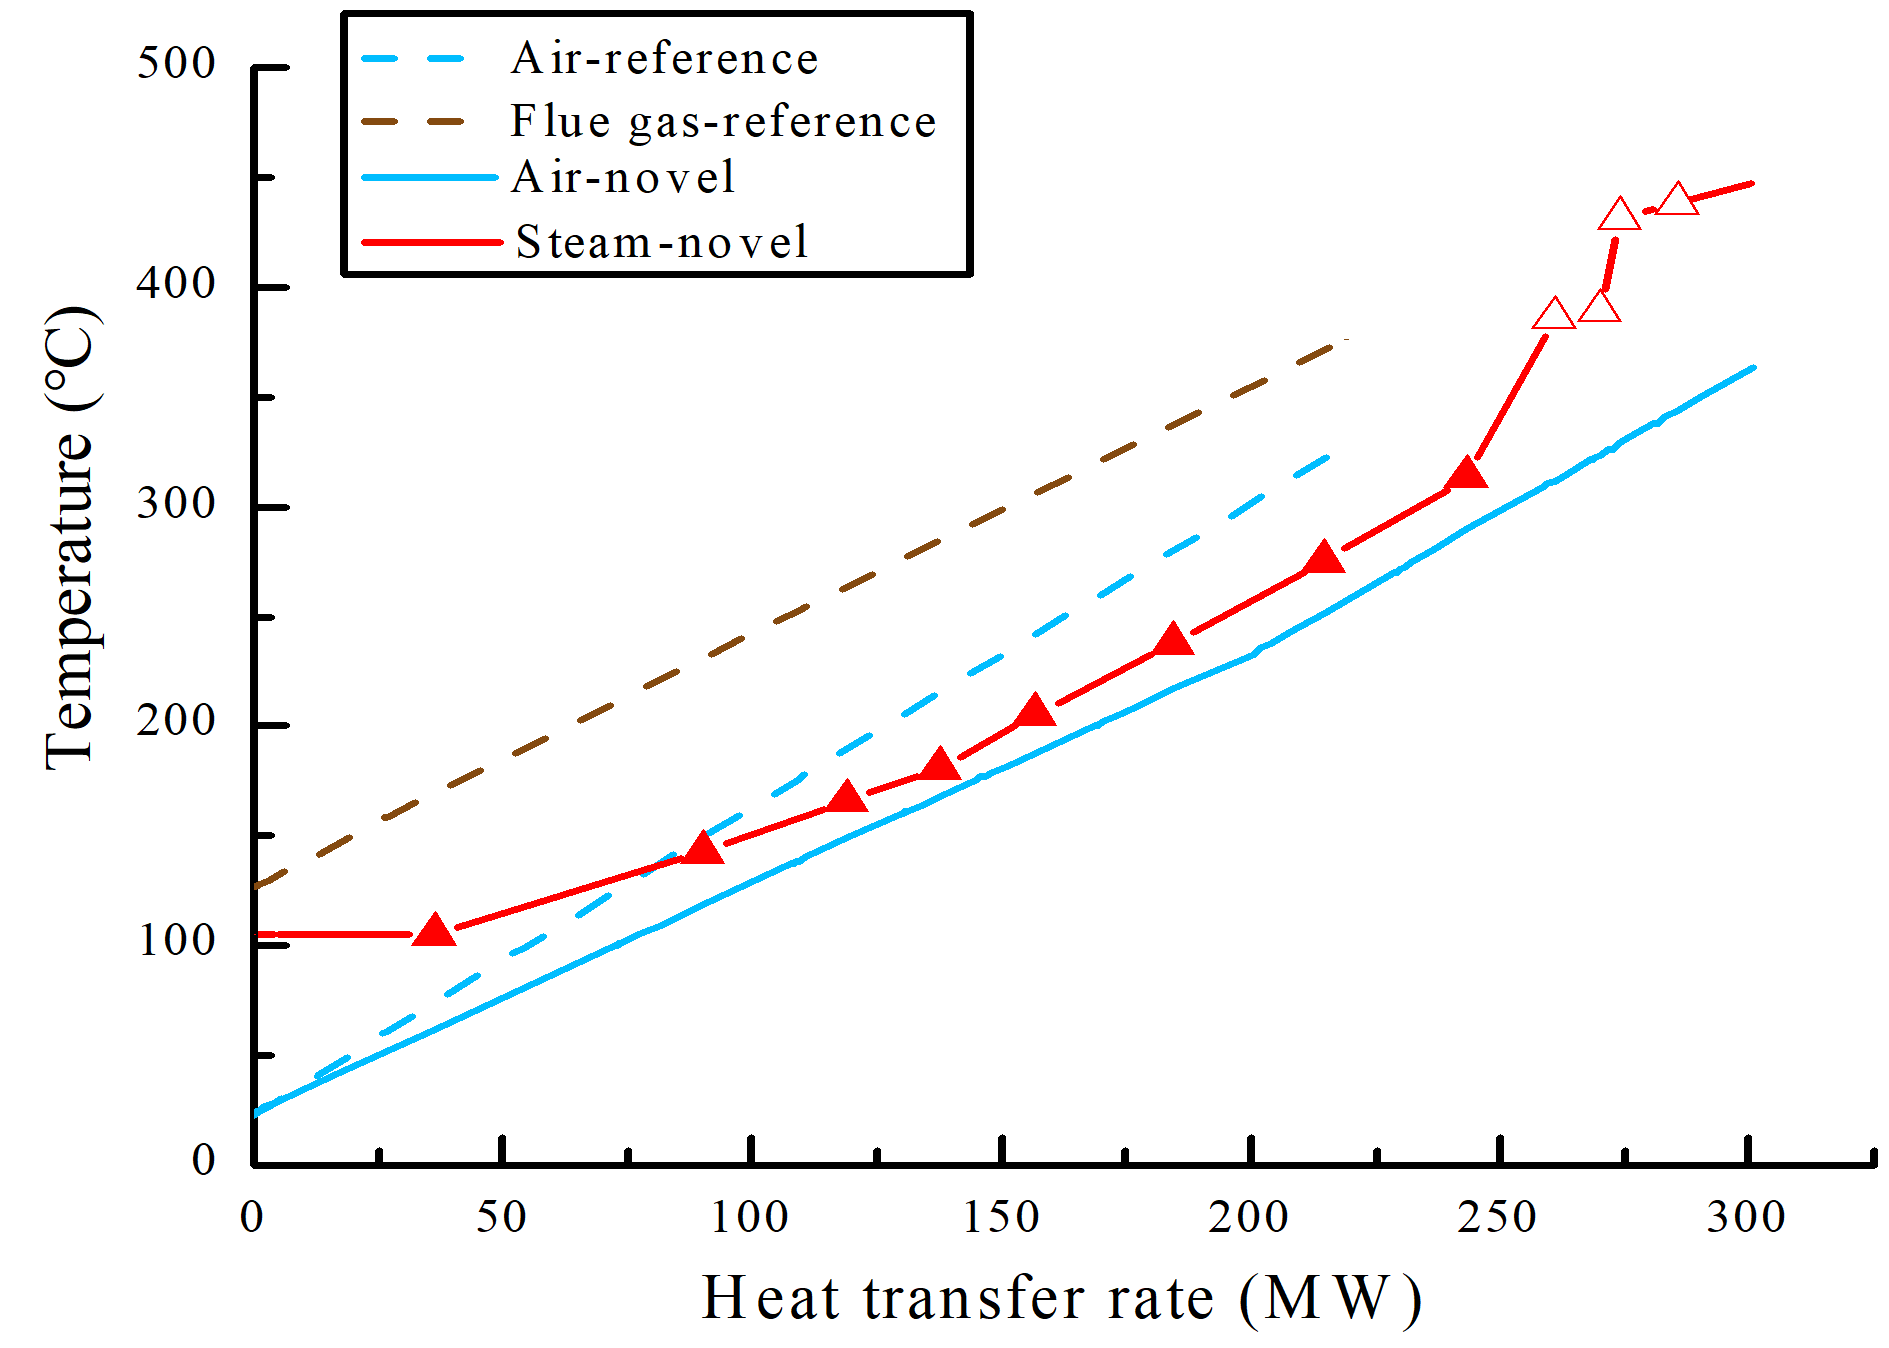
\includegraphics[width=0.6\textwidth]{fig/APH_temper_compare.png}
\caption{T-Q diagram of Air preheat subsystems} 
\label{fig:APH_temper_compare}
\end{figure}


Fig.~\ref{fig:APH_temper_compare} shows EAPHs and AOCs's exergy analysis results. 
Except EAPH8,the exergy efficiency of EAPHs and AOCs is higher than 82\%, and the APH8 has the greatest exergy loss and lowest efficiency of all the air preheaters. 
According with Fig.~\ref{fig:APH_temper_compare}, the heat transfer temperature difference of EAPH8 is 26.95 $^\circ$C,and it has a larger heat exchanging quantity, both of which cause higher exergy destruction and exergy efficiency.
It also indicates that, although the AOCs have large heat transfer temperature difference, their exergy efficiencies are still high and  exergy destruction rates are low.

Combing Fig.~\ref{fig:APH_temper_compare}  and Fig.~\ref{fig:novel_APH_exergy}, the reason why the novel system's air preheat subsystem have a higher exergy efficiency and lower exergy destruction rate can be drawn that the novel system's air preheat subsystem has a lower heat transfer temperature difference and reasonable extractions' superheat degree using.


\begin{figure}[htbp]
\centering
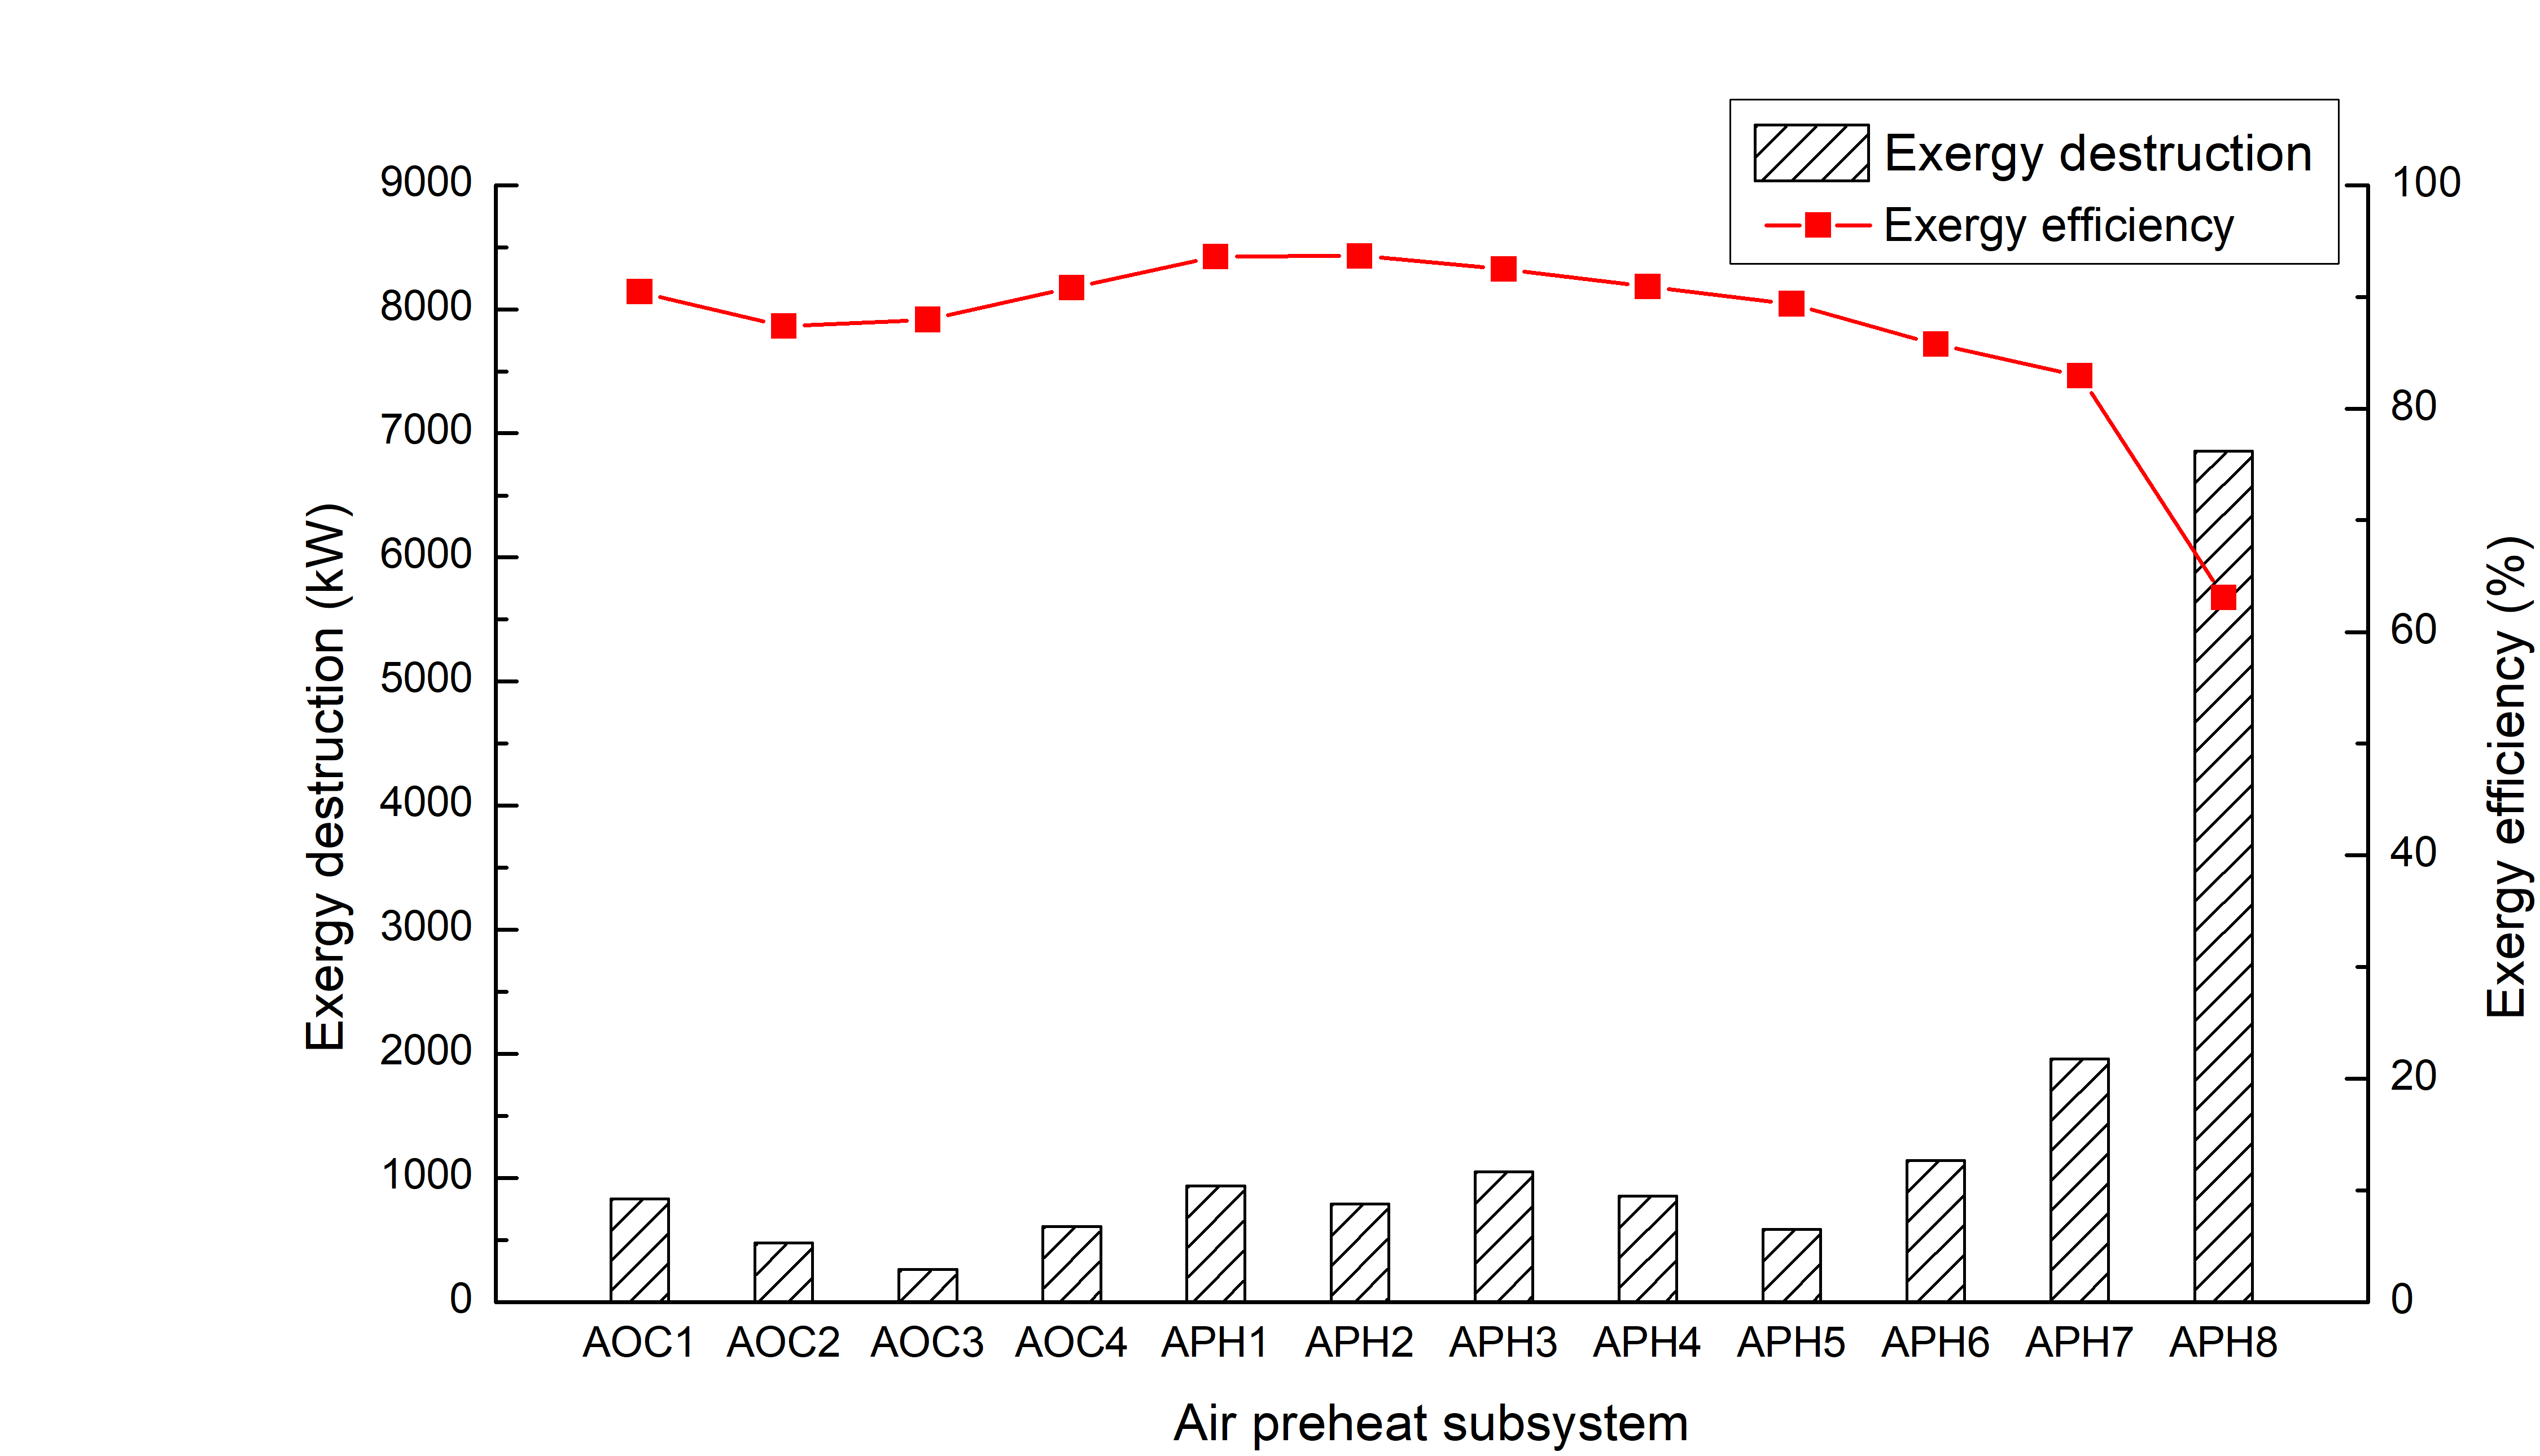
\includegraphics[width=0.8\textwidth]{fig/novel_APH_exergy.png}
\caption{Exergy destruction and efficiency of air preheat subsystem of novel system} %图中的纵坐标需要修改
\label{fig:novel_APH_exergy}
\end{figure}

The regenerative subsystem of novel system uses LEPS paralleled connected with EAPH to absorb economizer outlet flue heat, and eliminates the AOCs originally used to heat feedwater.
LPE inlet water are heated to the outlet temperature of corresponding RH outlet temperature of to mix up.
With the extractions' parameters keeping still, the average heat transfer temperature difference of RHs change little.
So their exergy efficiency keeps the same with reference system.

Fig.~\ref{fig:regenerative_subsys_compare} shows the regenerative subsystem's exergy destruction rate distribution comparison between the two systems.
It can be found that the novel system's exergy destruction rate has a decrease and great changes have taken place in the destruction's distribution.
In consequence of the flow diverting effects of LEPs, the exergy destruction rate of regenerative reheaters and DEA changes from 20.16 MW to 11.303 MW.
The LEPs exergy destruction rate reach to 10.25 MW, and Fig.~\ref{fig:LPE_exergy_LMDT} shows the LEPs' exergy efficiency and heat transfer LMTD.
As shown in Fig.~\ref{fig:LPE_exergy_LMDT}, the highest efficiency one is LPE1 with 93.50\%, and the lowest efficiency one is LPE4 with 87.44\%. 
The LEPs' overall exergy efficiency is 91.62\%, much higher than that of flu-air heat transfer of reference system, and the temperature difference of the LPEs is between 23$^\circ$C to 42$^\circ$C.

\begin{figure}[htbp]
\centering
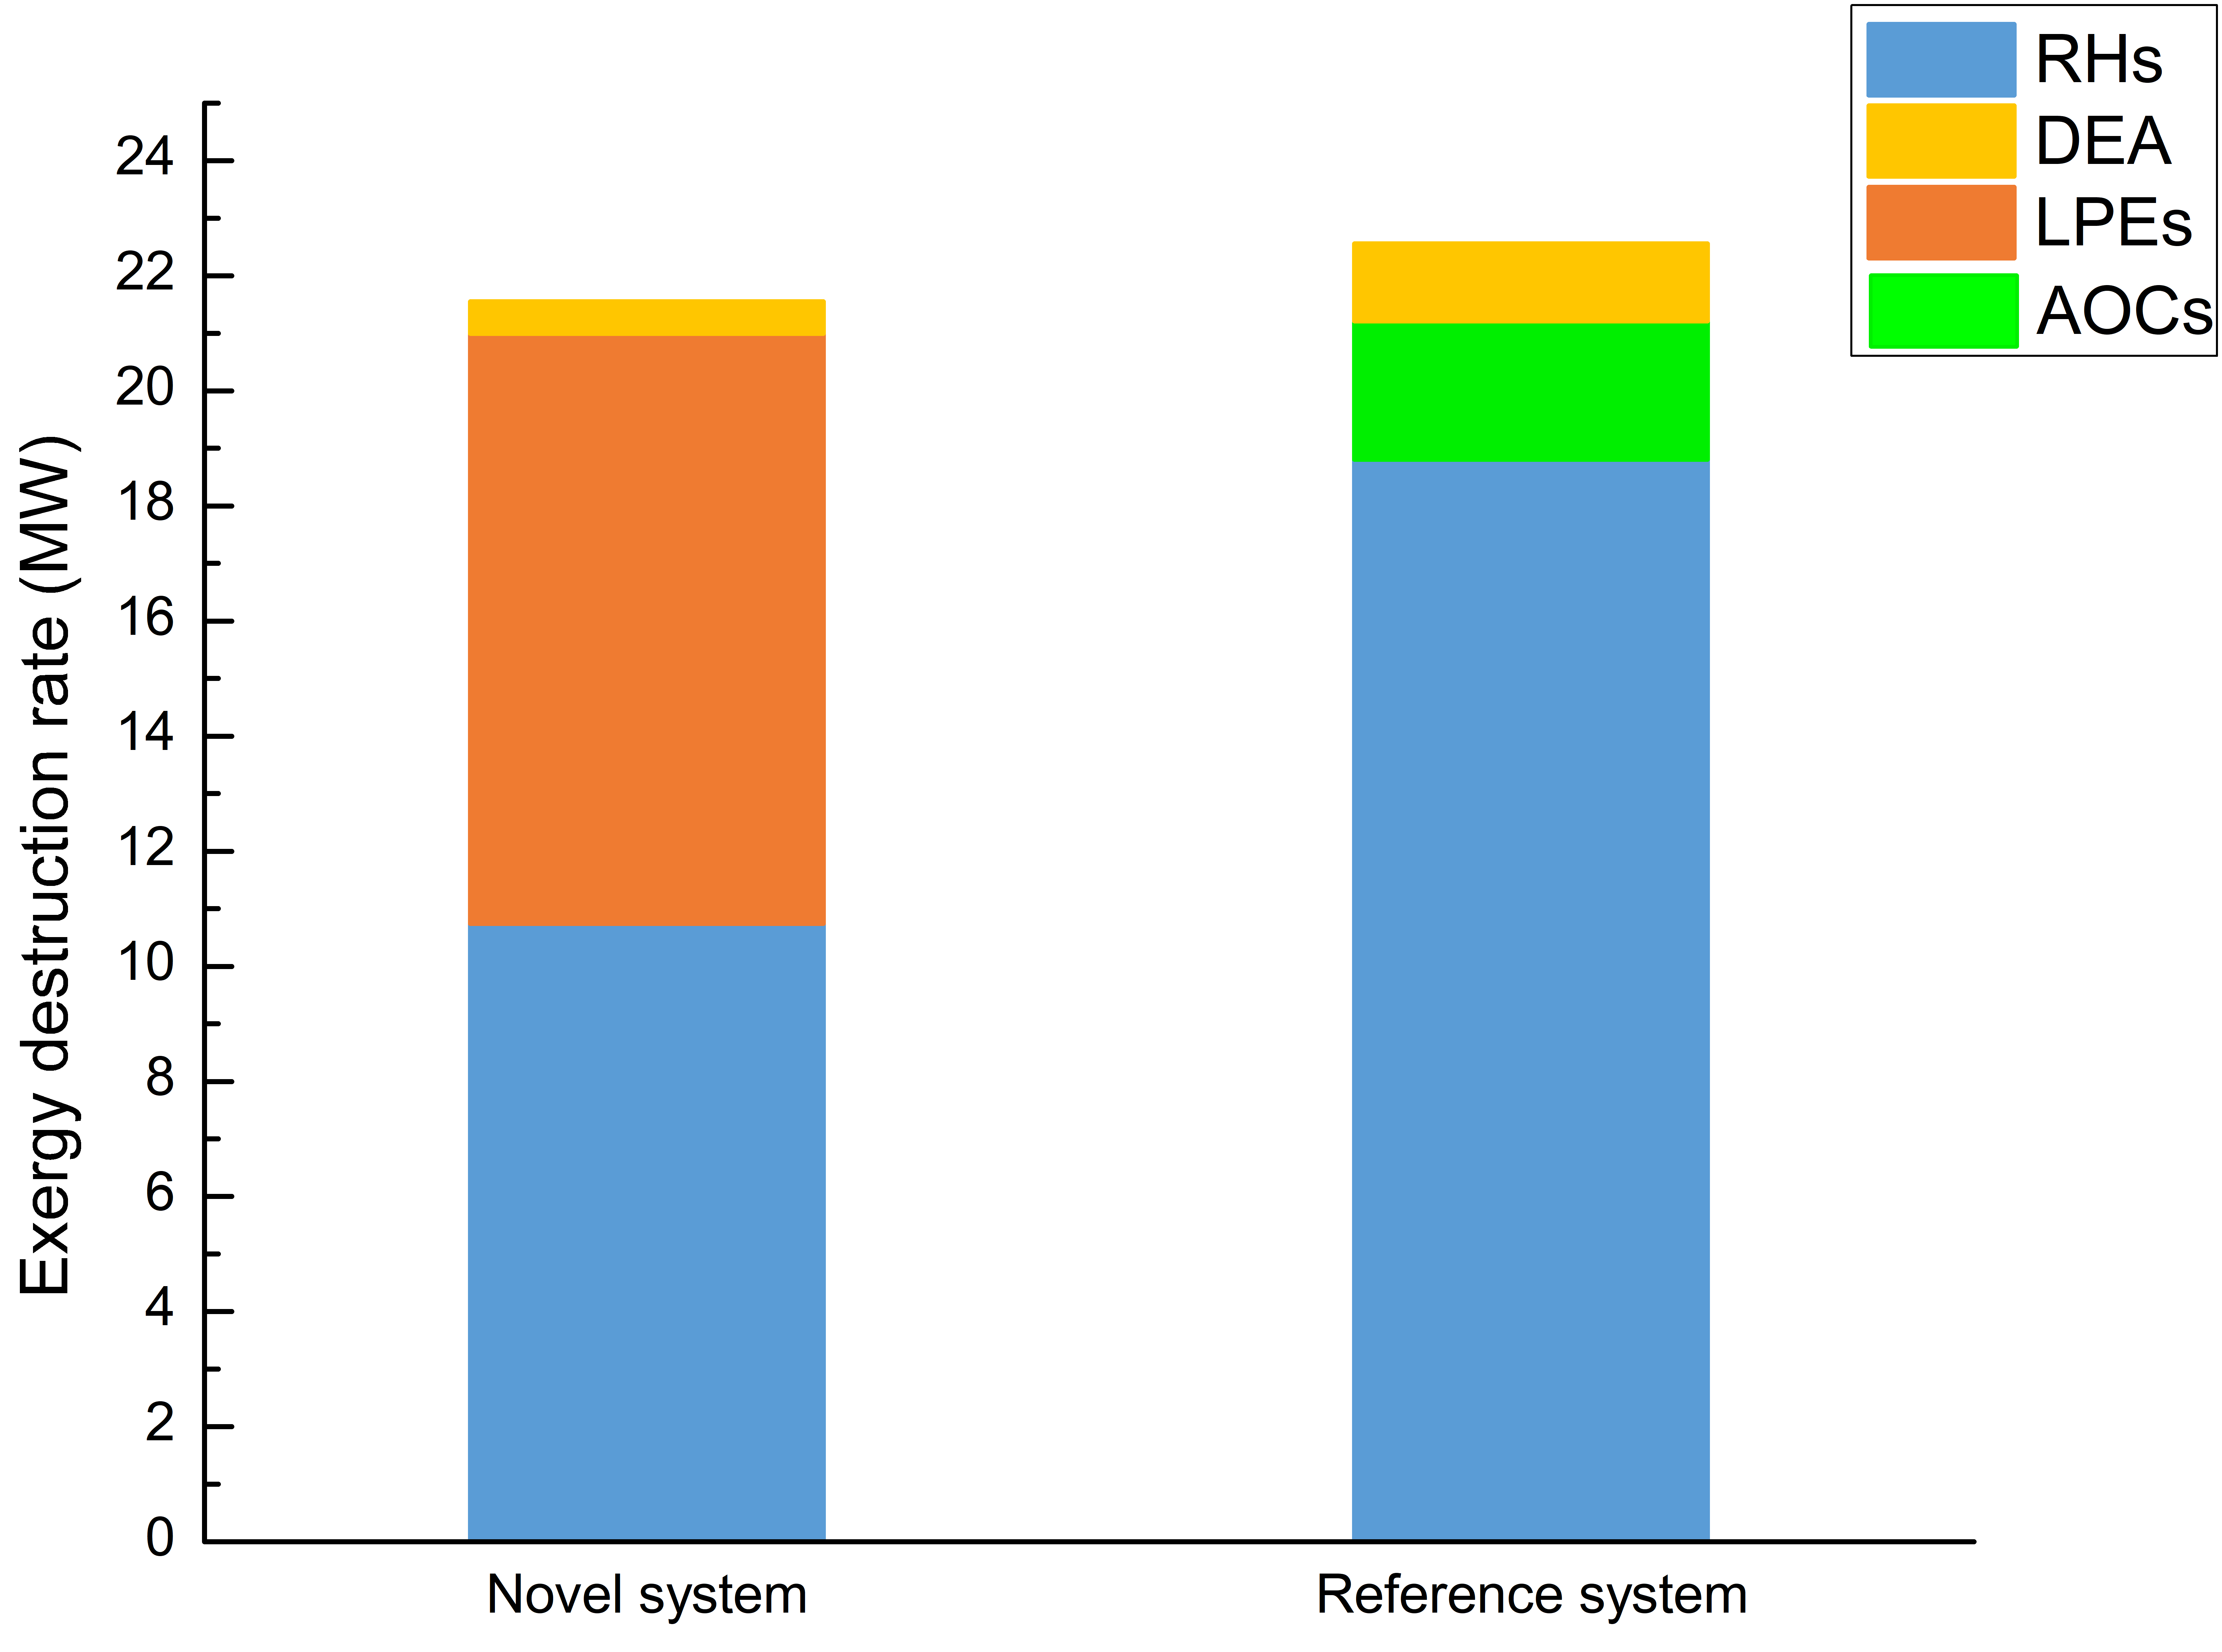
\includegraphics[width=0.6\textwidth]{fig/regenerative_subsys_compare.png}
\caption{Exergy destruction comparison of regenerative subsystems} 
\label{fig:regenerative_subsys_compare}
\end{figure}



\begin{figure}[htbp]
\centering
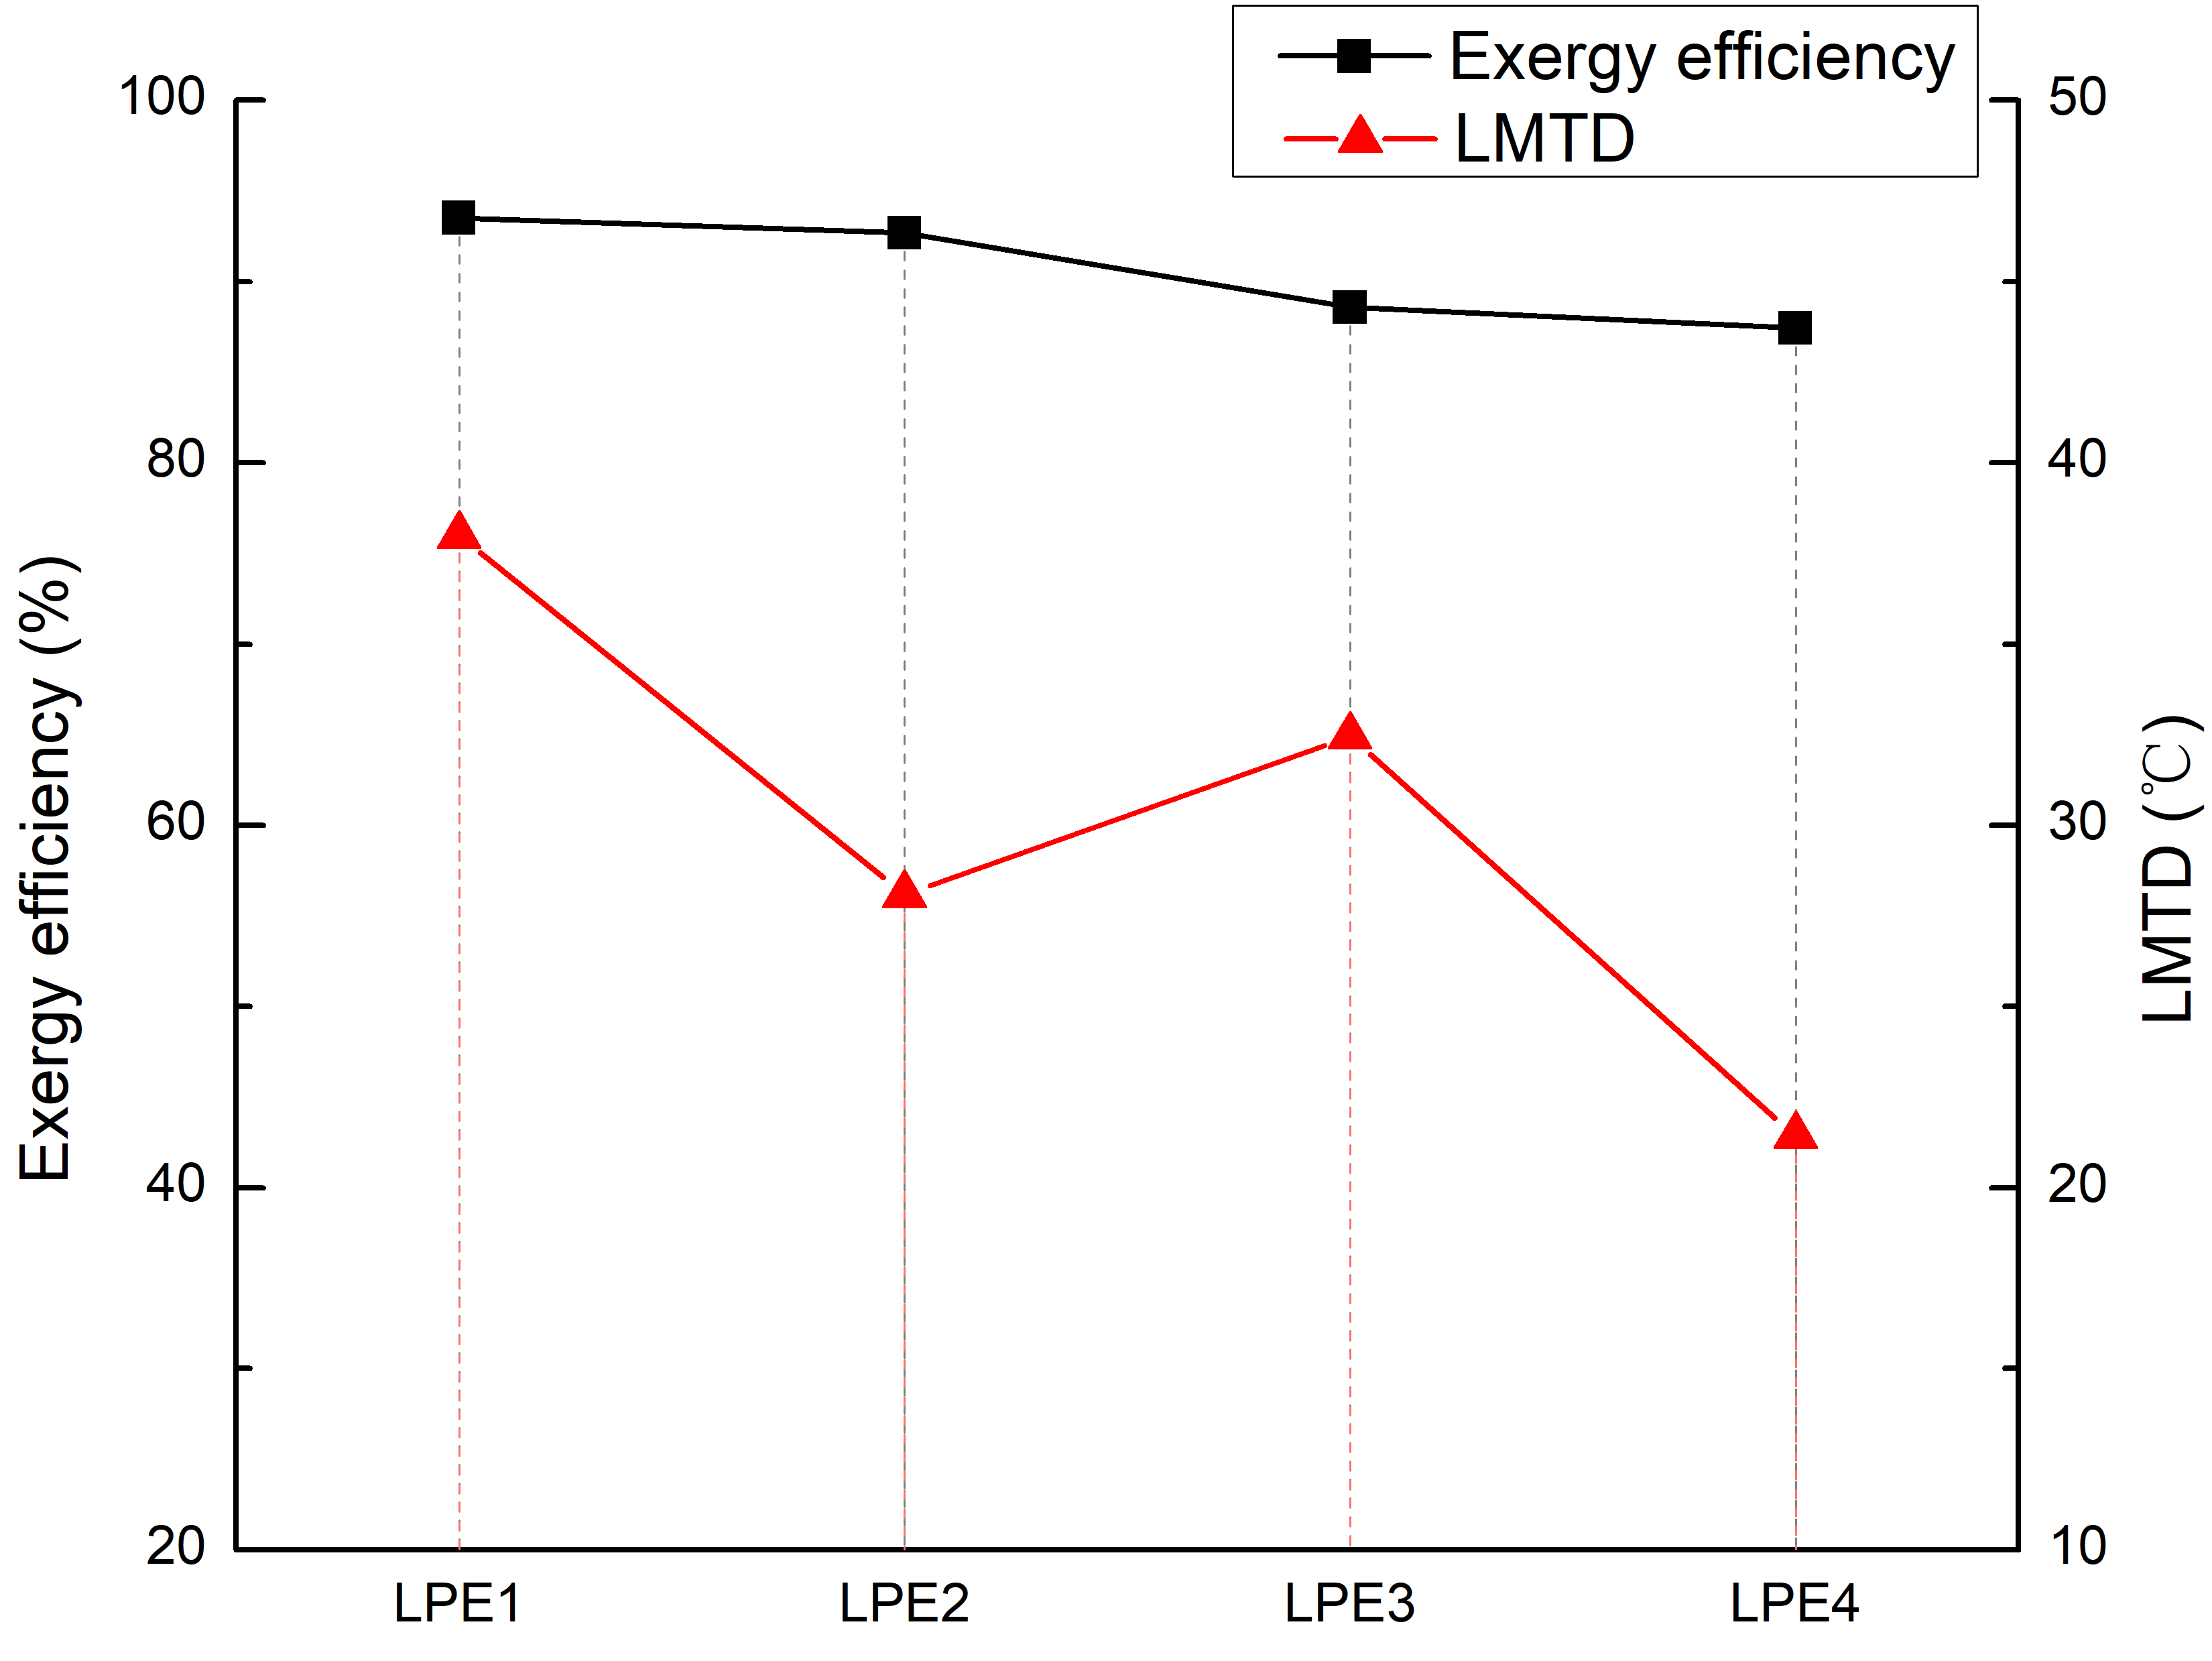
\includegraphics[width=0.6\textwidth]{fig/LPE_exergy_LMTD.png}
\caption{Exergy efficiency and LMTD of LPEs} 
\label{fig:LPE_exergy_LMDT}
\end{figure}


\subsection{Thermodynamic comparison in off-design conditions}
\label{ssub:offdesing_compare}
Considering that large USC power plants' operation under partial load conditions, it is necessary to study the thermal performance of double reheat USC power plants under off-design conditions.
Four typical operation conditions, THA load, 75\% THA load, 50\% THA load, and 40\% THA load conditions, were chosen for thermodynamic analyses. 
Fig.~\ref{fig:partload_efficiency} shows novel and reference systems' exergy efficiency under different load conditions.The exergy efficiencies of both systems decrease as the load decrease.
The exergy efficiencies of both systems are 47.52\% and 46.51\% under THA load condition. Compared with reference system, novel system's exergy efficiency has the increment of 1.01 percentage points, and reduces SCE consumption by 5.5\,g/kWh.
Under the 75\% THA condition, the optimized system was 46.56\% and the reference system was 45.90\%, the exergy
efficiency decrease to 0.66\%. 
When the load is equal to 50\% THA, the efficiency difference is 0.43\%.
This implies that the novel system can increase exergy efficiency under partial load, but it has more advantages for double reheat power plant undertaking base load.

\begin{figure}[htbp]
\centering
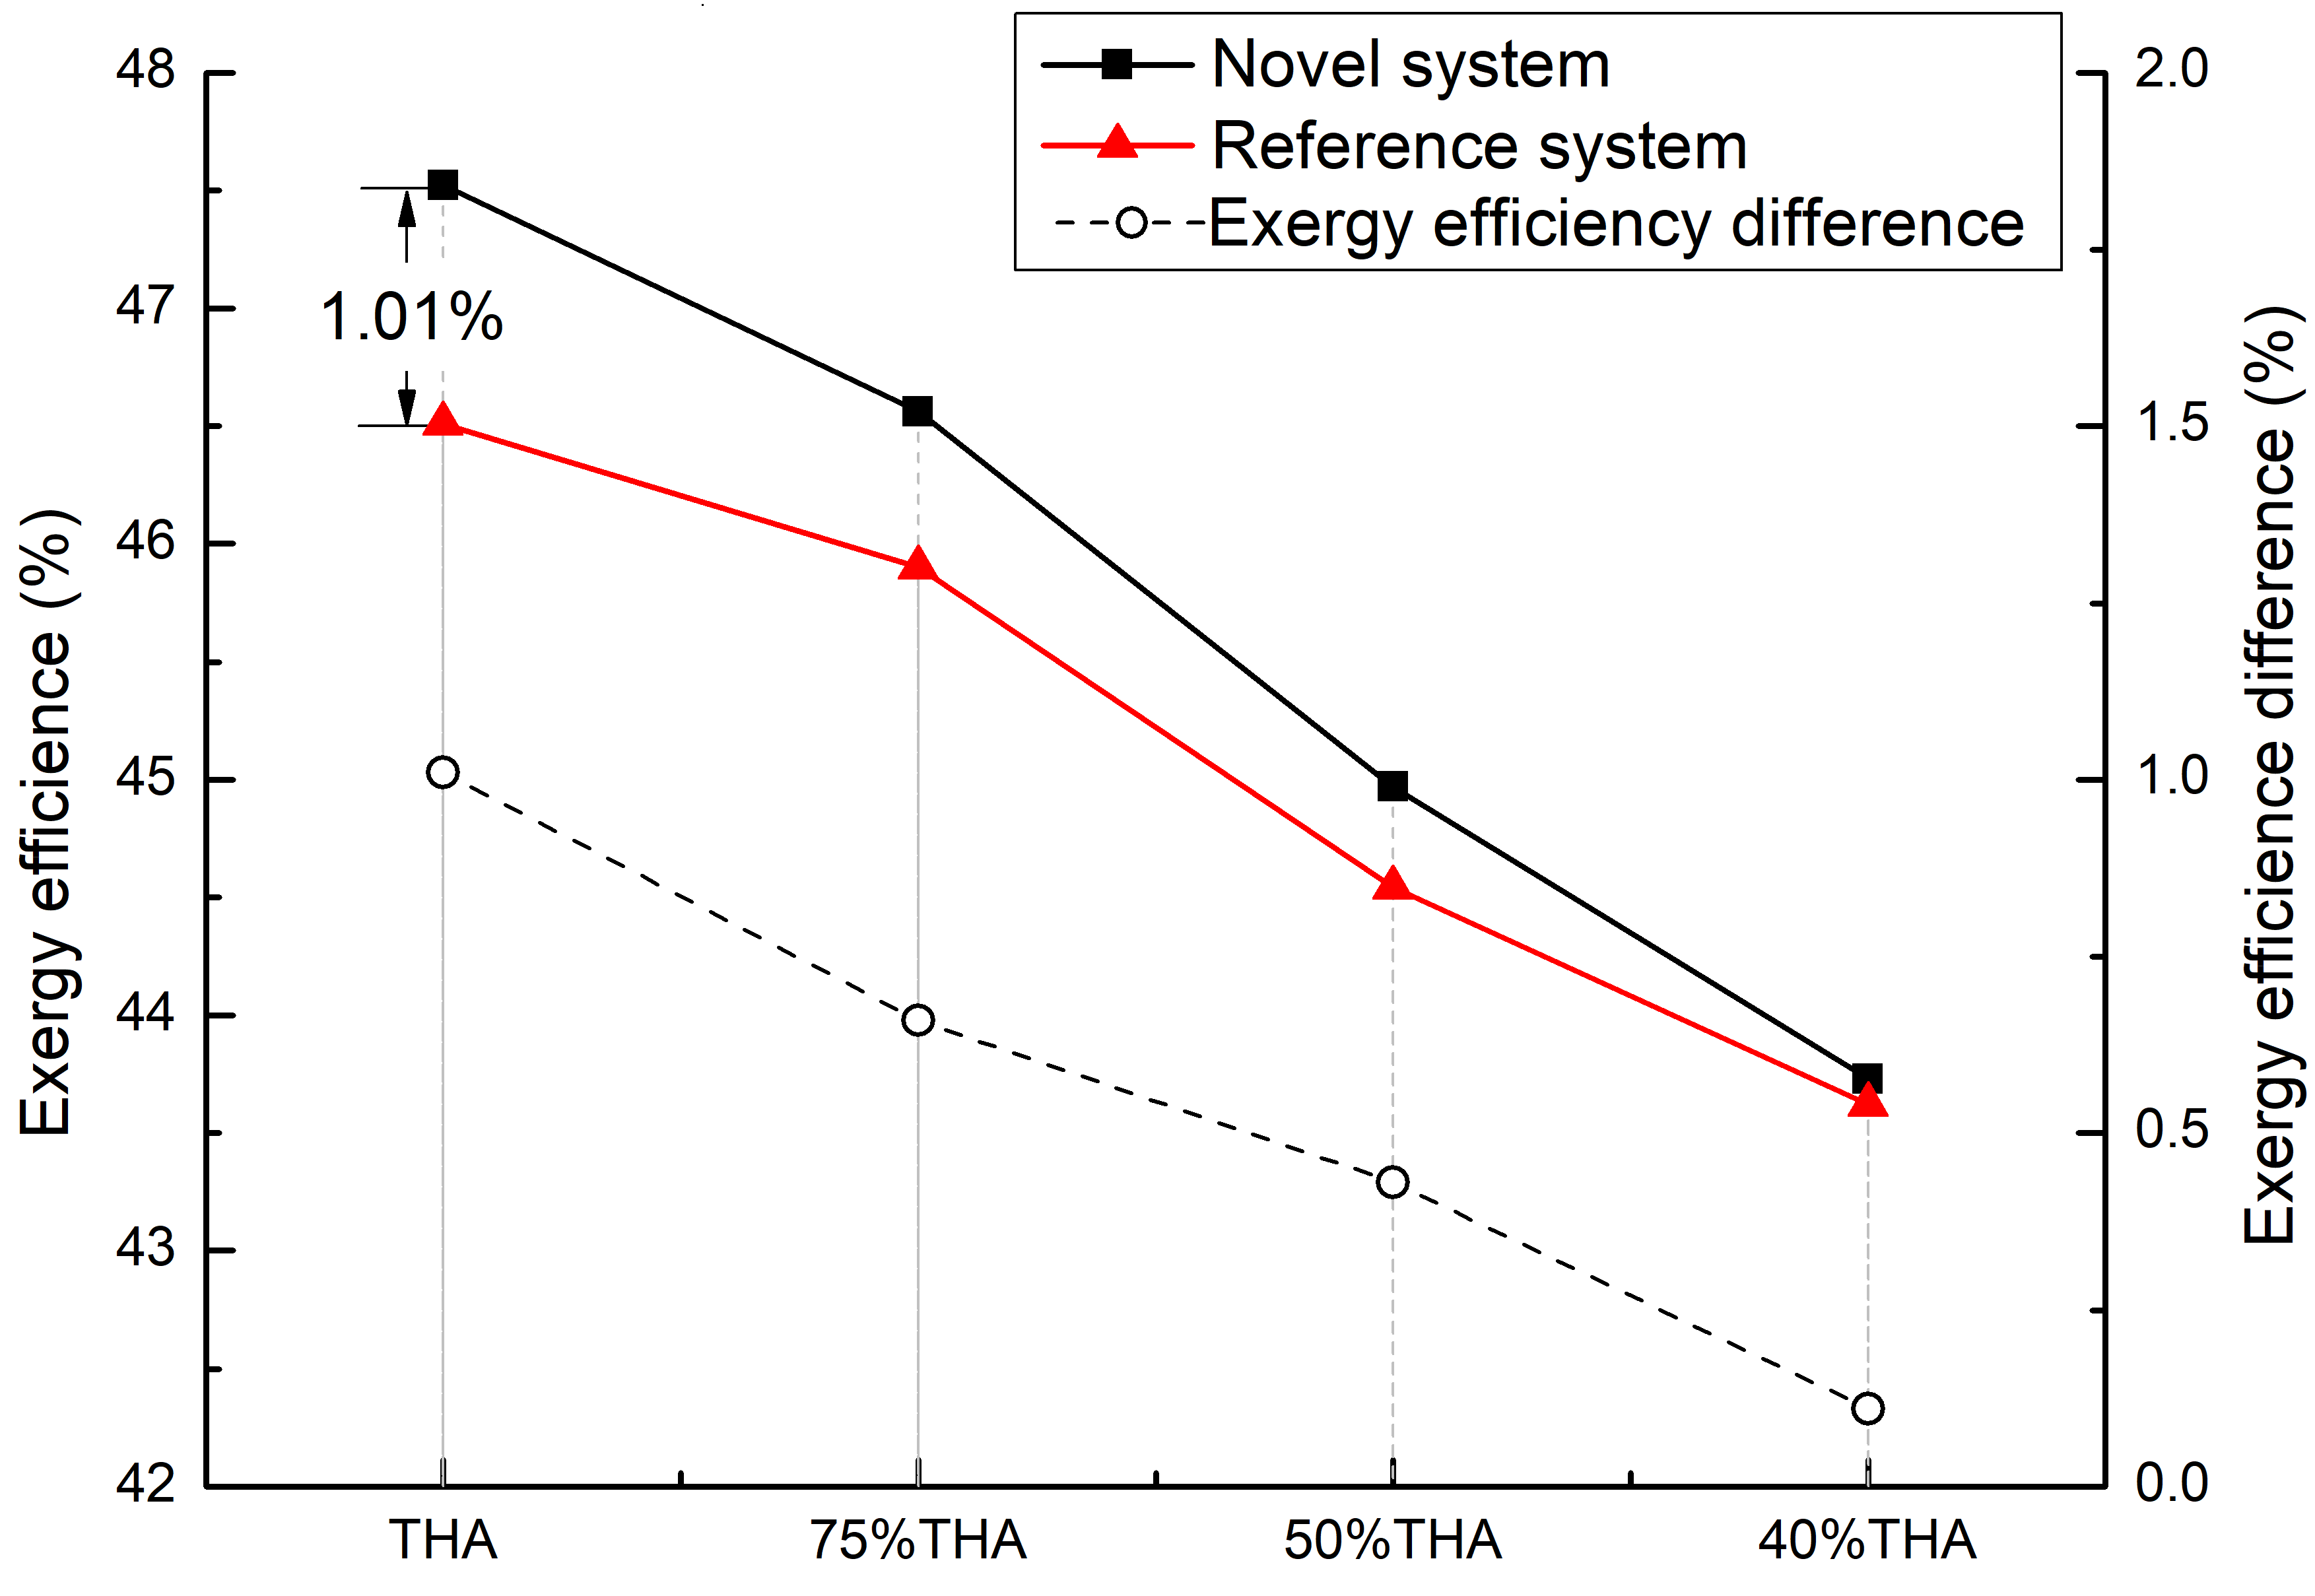
\includegraphics[width=0.6\textwidth]{fig/partload_efficiency.png}
\caption{Exergy efficiency comparison in off-design conditions} 
\label{fig:partload_efficiency}
\end{figure}
  exergy destruction ratio ($y_{D}$) is used to measure the exergy destruction of 1\,MW power generation of unit by a subsystem, and its calculate formula is as follow:
\begin{equation}
y_{D}=\frac{\dot{I}}{P}
\end{equation}

% 用损率差大表明该子系统的节能效果更显著,同时对整个系统的节能效果贡献更大。
% 由图10可以得到新系统引起节能效果从大到小依次为:锅炉、空预系统、回热系统和汽轮机。
% 当负荷从THA逐渐降低可以看到,降负荷对锅炉影响最大,而负荷变化对汽轮机系统影响接近于零。
% 负荷降低到40%,四个子系统优化效果虽然降低但累计值依然优于参考系统,但由于符合降低引起的oher系统用损失的升高导致优化系统相对与参考系统效率增加为0.01%,几乎没有优化效果
% 同时需要指出,由于锅炉本身的用损失很大,所以变负荷对锅炉本身用效率影响很小,而对空预子系统的影响较大。
A large exergy destruction ratio value indicates that the subsystem has more significant energy-saving effects and contributes more to the exergy-saving effect of the entire system.
Fig.~\ref{fig:partload_subsys_exergyrate} shows the  exergy destruction ratio difference ($y_{D,reference}-y_{D,novel}$) between reference system and novel system.
It indicates that the contribution of energy-saving effect decrease as follows: the boiler, air preheat subsystem, regenerative subsystem and steam turbine.
As the load decreases from THA load condition, it can be seen that the load change has the greatest effect on the boiler, while the change of load condition barely affects the steam turbine.
While the load is reduced to 40\%THA, the four subsystems of the novel system are still have lower exergy destruction rate than those of the reference system.
However the calculated value of these subsystem decrease and exergy destruction rate increase of other uncalculated components make the novel system's exergy-saving effect decrease.
According to the data of Table~\ref{table:system exergy campare}, it should be pointed out that due to the great exergy destruction of the boiler, the decrease of load has little effect on the exergy efficiency of it.But the air preheat subsystem is most effected.


\begin{figure}[htbp]
\centering
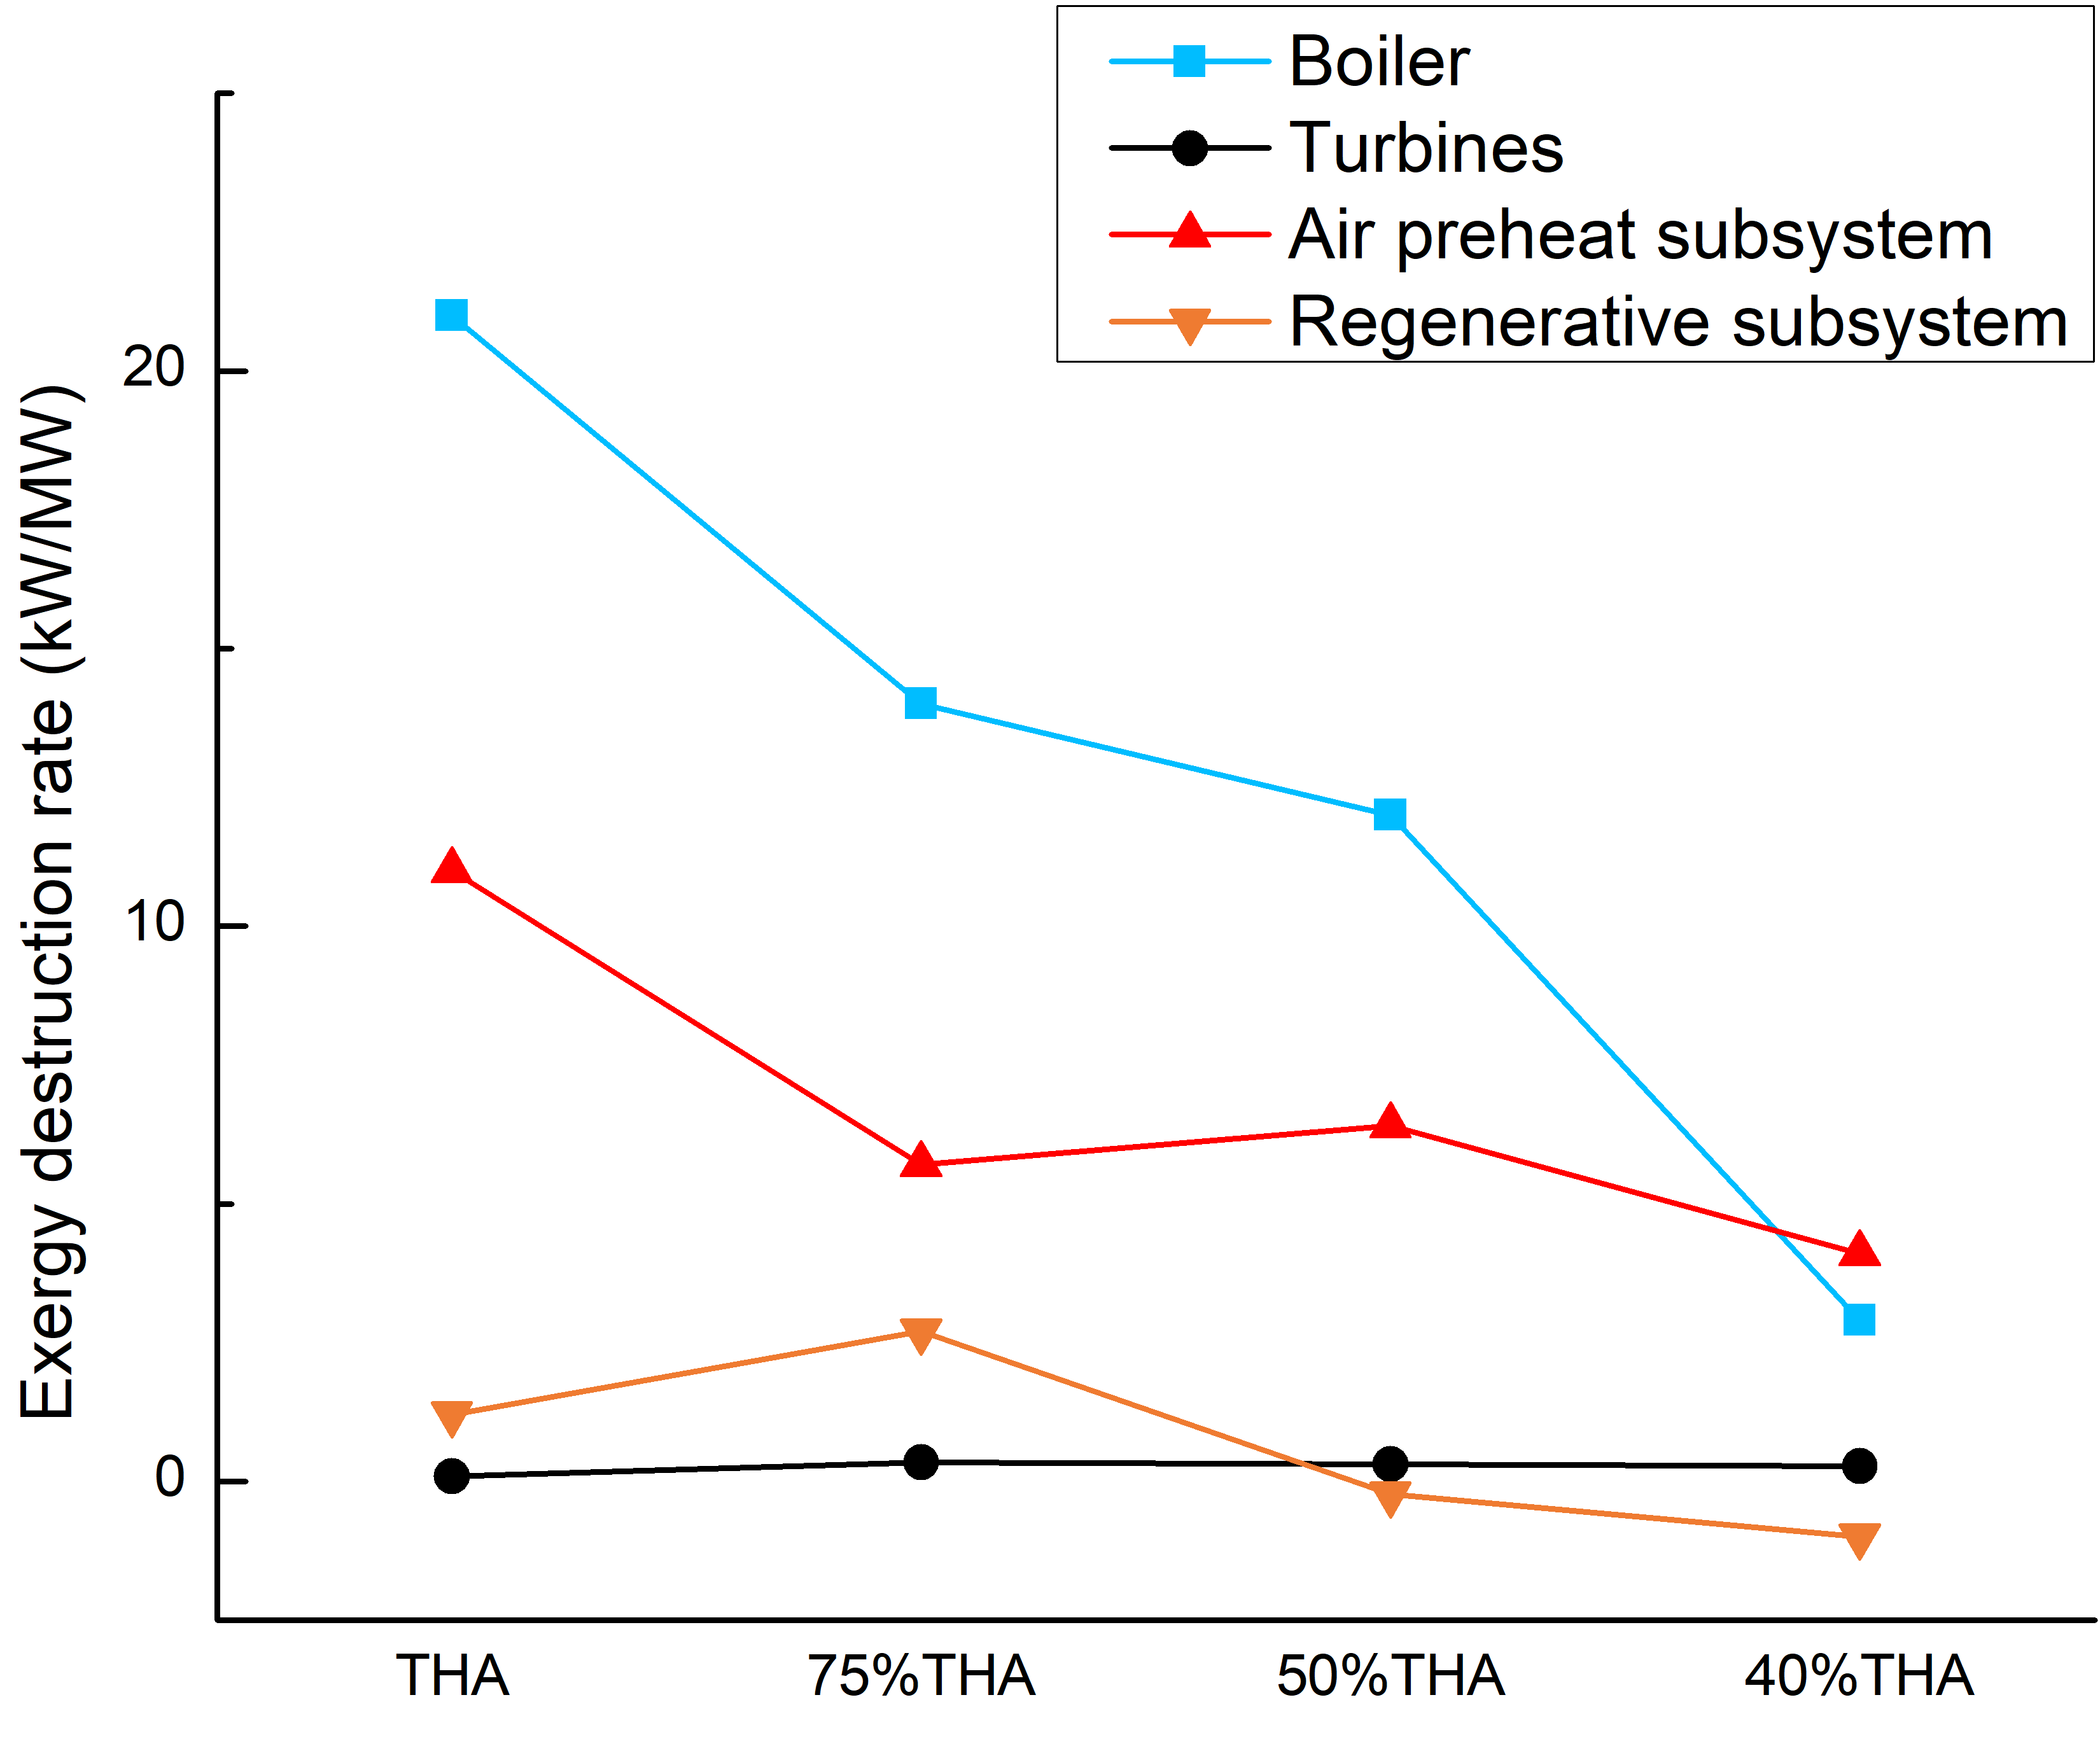
\includegraphics[width=0.6\textwidth]{fig/partload_subsys_exergyrate.png}
\caption{Exergy destruction rate difference of subsystems in off-design conditions} 
\label{fig:partload_subsys_exergyrate}
\end{figure}

% subsubsection subsubsection_name (end)

\section{Conclusion}
%文章干了什么
A novel system for a 1000\,MW double reheat ultra-supercritical unit is proposed which use turbine extractions to preheat air and low pressure economizers to replace air preheater originally installed in vertical shaft.
Thermodynamic analysis is conducted to reveal the energy-saving effects and thermal performance changes of key components. 
The novel system is found to be effective in overcoming the imperfections, and may provide an effective method for the optimization of  double reheat USC unit.
The following conclusions are drawn from this study: 
 \begin{enumerate}[(1)]
 \item The novel system can improve power generation efficiency to 48.73\%, which is 1.04 percent higher then the reference system under design condition.And the exergy efficiency of novel system is 47.52\%, which is 1.01 percentage higher then the reference system.
 \item The thermodynamic analysis indicates that the novel system decreases the temperature difference of air/flue-gas heat transfer process which achieves the cascaded utilization of energy, and the superheat degree of the 3rd and 5th is reduced greatly. 
\item The novel system changes the mass flow rates distribution of extractions, which causes increment of output power of the generator by 12.09 MW 
\item The novel system improves the temperature of secondary air, which improves the fire condition in the combustion chamber.
 The temperature of secondary air of reference system under full load is 365$^\circ$C, which is 34$^\circ$C higher than the reference system.
\item The novel system theoretically brings remarkable energy saving effects even under off-design conditions. The simulation results show that the optimization system can reduce the SCE consumption by 5.49 g/kWh under design condition, and can even bring a reduction of 2.9 g/kWh under 50\% THA load.
\end{enumerate}
\section*{Acknowledgments}
This study is supported by National Basic Research Program of China (Grant No. 2015CB251504).
\section*{References}
\bibliographystyle{elsarticle-num}

\bibliography{bib/reference.bib}


\nomenclature[M]{$\dot{I}$}{exergy destruction rate (MW)}%
\nomenclature[M]{$\dot{Ex}$}{exergy rate (MW)}%
\nomenclature[M]{$\dot{W}$}{work rate or power done by the system (MW)}%
\nomenclature[M]{$\eta_{\uppercase\expandafter{\romannumeral2}}$}{exergy efficiency}%y D
\nomenclature[M]{$y_{D}$}{exergy destruction ratio (MW/MW)}

\nomenclature[M]{$ex$}{specific exergy (MJ/kg)}%

\nomenclature[M]{$h$}{specific enthalpy (MJ/kg)}%
\nomenclature[M]{$s$}{specific entropy (MJ/kg\,K)}%
\nomenclature[M]{$T$}{temperature (K)}%
\nomenclature[M]{$\dot{m}$}{mass flow rate (kg/s)}%

\nomenclature[S]{$in$}{inlet component or system}%
\nomenclature[S]{$out$}{outlet component or system}%




\nomenclature{THA}{turbine heat acceptance}

\nomenclature{AOC}{additional outer steam cooler}
\nomenclature{SCE}{standard coal equivalent}
\nomenclature{USC}{ultra-supercritical}
\nomenclature{LPE}{low pressure economizer}
\nomenclature{EAPH}{turbine-extraction-heated air preheater}
\nomenclature{APH}{air preheater}

\nomenclature{VHP}{super high pressure cylinder}
\nomenclature{HP}{high pressure cylinder}
\nomenclature{IP}{intermediate pressure cylinder}
\nomenclature{LP}{low pressure cylinder}
\nomenclature{ECO}{ economizer}

\nomenclature{RH}{regenerative heater}
\nomenclature{HRH}{high pressure regenerative heater}
\nomenclature{LRH}{low pressure regenerative heater}
\nomenclature{DEA}{deaerator}



\nomenclature{LMTD}{logarithm mean temperature difference} 
\nomenclature{LHV}{lower heating value of fuel} 

\nomenclature{C, H, O, N}{mass fraction of carbon, hydrogen, oxygen, nitrogen of coal} 

\end{document}

\endinput
\%\%
\%\% End of file `article.tex'.
